% Created 2025-06-29 Sun 15:21
% Intended LaTeX compiler: pdflatex
\documentclass[11pt]{article}
\usepackage[utf8]{inputenc}
\usepackage[T1]{fontenc}
\usepackage{graphicx}
\usepackage{longtable}
\usepackage{wrapfig}
\usepackage{rotating}
\usepackage[normalem]{ulem}
\usepackage{amsmath}
\usepackage{amssymb}
\usepackage{capt-of}
\usepackage{hyperref}
\usepackage{enumitem}
\usepackage{pgfplots}
\usetikzlibrary{arrows}
\usepackage{xcolor}
\definecolor{pourpre}{HTML}{CCCCFF}
\definecolor{citron}{HTML}{BFFF00}
\usepackage[french]{babel}
\usepackage[colorlinks=true, linkcolor=blue]{hyperref}
\author{Laurent Garnier}
\date{2025}
\title{Exercices de calculs et représentations géométriques}
\hypersetup{
 pdfauthor={Laurent Garnier},
 pdftitle={Exercices de calculs et représentations géométriques},
 pdfkeywords={},
 pdfsubject={Livre d'exercices progressifs en calcul mental, algèbre, géométrie, probabilités et statistiques du primaire au lycée.},
 pdfcreator={Emacs 29.4 (Org mode 9.6.15)}, 
 pdflang={French}}
\begin{document}

\maketitle



\section{Introduction}
\label{sec:orgbdfe192}

Ce livre a pour but de vous faire faire des mathématiques. 

On commence par du calcul mental afin d’échauffer l’esprit. Oui, même
au XXI\up{e} siècle, alors que nous avons des calculatrices, des
ordinateurs, des téléphones et même des intelligences artificielles,
il est encore utile d’exercer son cerveau sur ce genre de tâches. Loin
de moi l’idée de vous prendre pour des calculateurs, ni d’essayer de
vous entraîner à le devenir : je n’en suis pas un, et j’aurais du mal
à vous entraîner pour ce genre de compétitions. Mais, de la même façon
que les humains n’ont pas cessé de marcher et de courir après
l’invention de la voiture, de l’ascenseur et des autres moyens de
transport, il en va de même pour l’exercice cérébral. Sans être
médecin, il me semble que le bon sens nous dicte que, si l’on reste
assis sur le canapé à manger de la malbouffe sans faire de sport, il y
a de gros risques de rencontrer des problèmes de surpoids et de santé
en général. L’exercice cérébral est une gymnastique de l’esprit :
c’est une hygiène mentale.


Néanmoins, il serait vain — et surtout ennuyeux — de se cantonner aux
calculs. L’activité mathématique est bien plus riche que cela. Il ne
s’agit pas de comptabilité. Même si l’arithmétique et le calcul
algébrique restent des outils cruciaux dans l’architecture des
mathématiques, les maths ne se résument pas à des calculs. D’un autre
côté, oublier cet aspect serait une carence aussi flagrante que celle
d’un sportif de haut niveau (footballeur, nageur, judoka… choisissez
votre sport favori) qui ne ferait pas de musculation. Les sportifs
font de la musculation parce que leurs muscles sont leurs outils pour
accomplir leur art. En mathématiques, c’est pareil : les calculs et la
capacité à les conduire sont utiles pour résoudre des problèmes
mathématiques.


Ce livre s’articule en trois parties principales, en plus de cette
introduction.


La première partie doit être faite par tous les lecteurs en guise
d’échauffement. Il s’agit de calculs \frquote\{\textit{purs et durs}\},
de niveau primaire. En effet, l’école primaire a pour but de faire
acquérir la maîtrise des quatre opérations de l’arithmétique de base,
à savoir : addition, soustraction, multiplication et division. Cela
peut paraître simple, mais derrière ces \frquote\{\textit{simples}\}
opérations se cachent les structures algébriques que nous aborderons
dans un prochain ouvrage consacré à l’enseignement supérieur.


Dans la seconde partie, on passe au niveau collège, en ajoutant des
calculs de carrés, des programmes de calculs, le calcul littéral, les
liens entre géométrie et calcul, et des probabilités de base en termes
de rapports d’aires de figures élémentaires.


Enfin, dans la troisième partie, on passe au niveau lycée :
configurations de nombres, vecteurs, statistiques et situations
concrètes.


Le souhait de cet ouvrage est de fournir des exercices faisables
directement, sans avoir à \textit{réviser le cours}. Trop souvent
aujourd’hui, les élèves sont traumatisés par la crainte de ne pas
connaître \frquote\{\textit{la phrase du cours}\}, comme s’il s’agissait
d’une incantation magique. Aucun cours de mathématiques n’est tombé du
ciel, telles les tables de la Loi. L’activité mathématique s’est
développée au cours des siècles à travers des problèmes qui, une fois
résolus, ont donné lieu à des généralisations, lesquelles sont ensuite
devenues des cours. Alors bien sûr, on ne peut pas se permettre le
luxe de tout redémontrer à partir de zéro, sinon chaque génération
aurait à refaire tout ce qu’a fait la précédente. Néanmoins, il me
semble beaucoup plus intéressant, et surtout utile et efficace, de
s’exercer d’abord ; et, à force de pratique, le cours pourra alors
être vu comme quelque chose d’intéressant… un nouveau genre
d’exercice.


Ma critique première est que les enseignements primaires et
secondaires (surtout primaire et collège) manquent cruellement de
démonstrations (alors que des démonstrations géométriques de base sont
accessibles très tôt), au profit d’un apprentissage par cœur dénué de
raisonnement et de réflexion, destiné à créer des
\textit{automatismes}. À l’époque de l’intelligence
artificielle, il me semble d’autant plus absurde de vouloir former des
générations d’automates, déjà dépassés par les véritables
automates. Nous, humains, faisons des erreurs et avons la capacité
d’apprendre de nos erreurs. C’est précisément pour cette raison qu’il
faut cultiver l’art de se tromper intelligemment.


L’art de se tromper intelligemment signifie prendre le risque de
pousser un raisonnement jusqu’à son terme, pour se rendre compte s’il
fonctionne ou non. Comprendre signifie prendre un risque : sans prise
de risque, vous ne pourrez jamais comprendre ; sans erreur, vous ne
pourrez jamais comprendre.


Ici, tous les exercices sont corrigés, donc vous pouvez les faire en
toute honnêteté, en prenant véritablement le risque de vous
tromper. De plus, pour la plupart des exercices (en dehors de ceux de
calculs purs), il y a souvent plusieurs façons de les résoudre. Il ne
faut donc pas chercher à mémoriser les corrections.


Les exercices sont presque tous originaux ou des adaptations de classiques.

\newpage

Pour toutes remarques, suggestions, ou demandes d'aide personnelles
merci de remplir \href{https://forms.gle/x7fAce7GqiJAGbsC7}{ce formulaire}.


\newpage

\section{Un peu de culture historique}
\label{sec:org75c9f53}
\subsection{Origine étymologique du mot calcul}
\label{sec:orgd9a48b2}

\begin{figure}[htbp]
\centering
\includegraphics[width=0.75\textwidth]{./images/Cailloux.jpeg}
\caption{Cailloux utilisés pour le calcul dans l'Antiquité}
\end{figure}



Le mot \textbf{calcul} vient du latin \textbf{calculus}, qui signifiait littéralement "petit caillou".
Ce terme dérive de \textbf{calx, calcis} (chaux, pierre calcaire).
Les Romains utilisaient effectivement de petits cailloux ou jetons pour effectuer leurs opérations arithmétiques sur l'abaque.

\newpage

\subsection{Premières traces de calculs}
\label{sec:org2012972}

\subsubsection{Os d'Ishango (\textasciitilde{}20 000 ans)}
\label{sec:orgb2c2681}

\begin{figure}[htbp]
\centering
\includegraphics[width=0.25\textwidth,height=5cm]{./images/Os-Ishango.jpeg}
\caption{Os d'Ishango (RDC)}
\end{figure}


Ces os, appelés bâtons d'Ishango, sont considérés comme les plus
anciens outils de calcul connus.

Découverts dans l’actuelle République Démocratique du Congo, ils
datent de plus de 20 000 ans.




\subsubsection{Jetons d’argile mésopotamiens (\textasciitilde{}8000-3000 av. J.-C.)}
\label{sec:org7847ca6}

\begin{figure}[htbp]
\centering
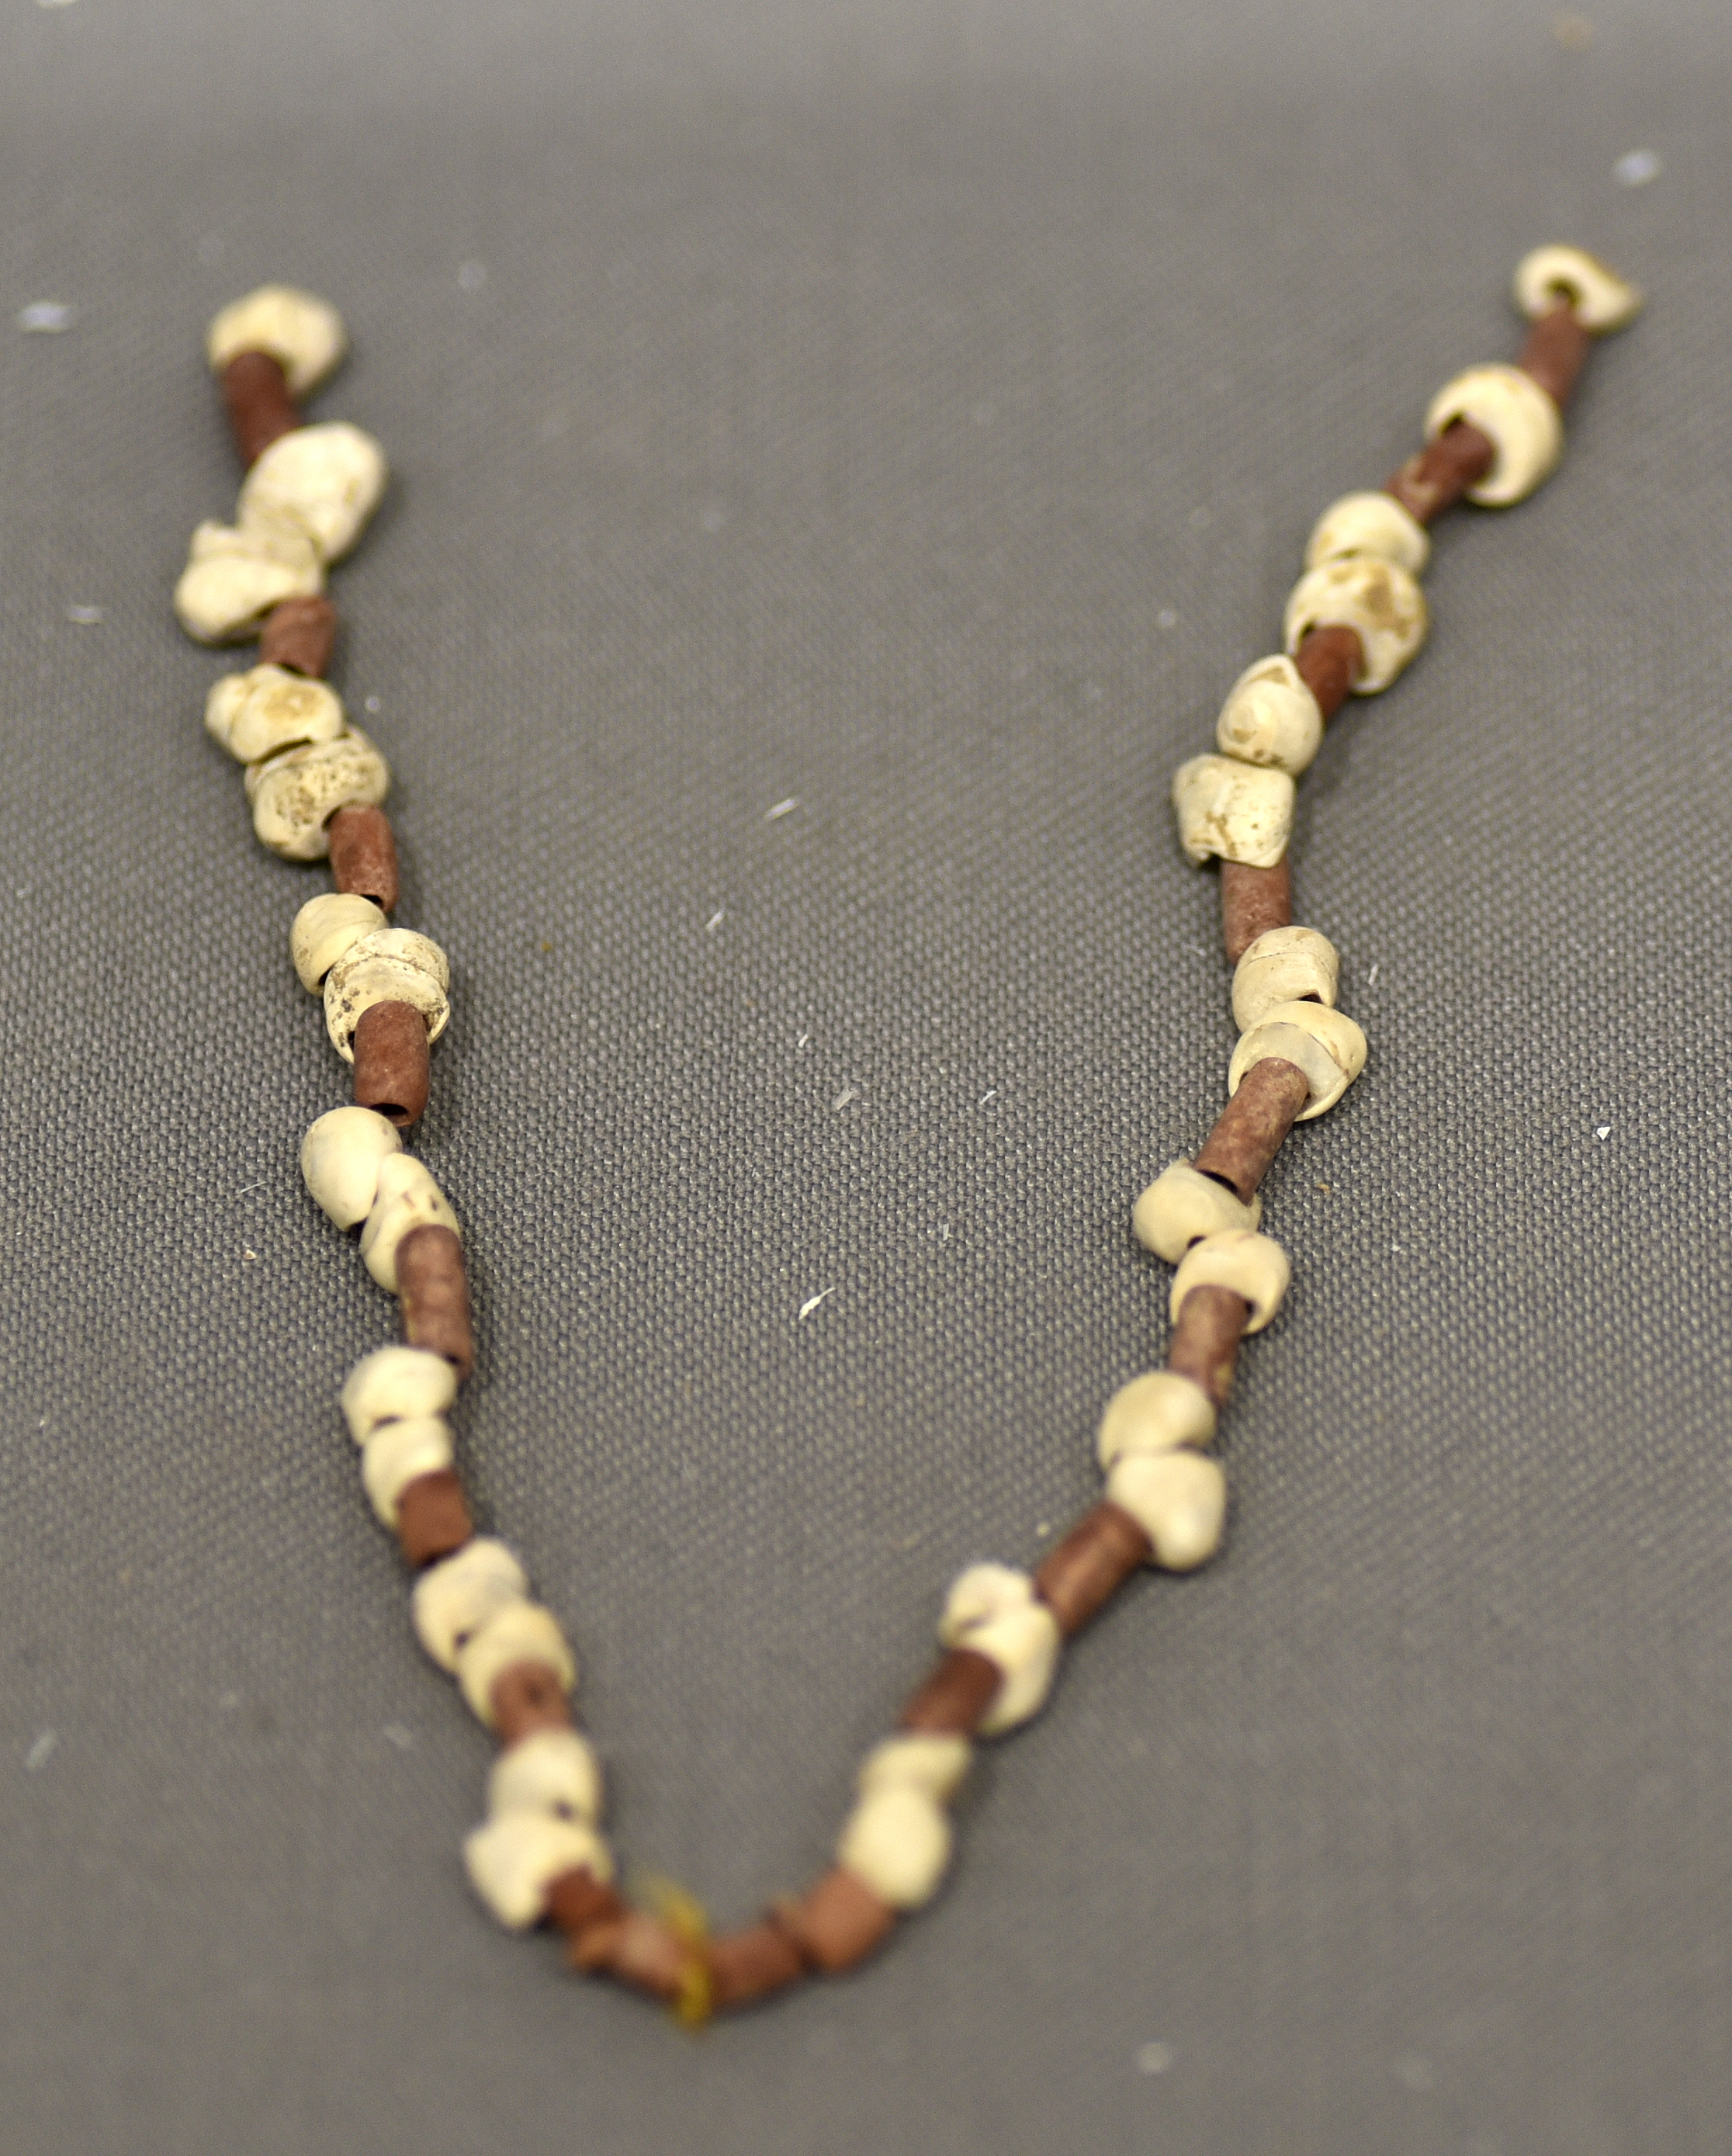
\includegraphics[width=0.25\textwidth,height=5cm]{./images/collier7800.jpg}
\caption{Jetons d’argile mésopotamiens}
\end{figure}



Ces petits objets servaient à compter les biens (bétail, céréales)
avant l’écriture.

Ils sont à l’origine des premiers systèmes comptables.



\subsubsection{Tablettes cunéiformes babyloniennes (\textasciitilde{}3000 av. J.-C.)}
\label{sec:orgdb3bf21}

\begin{center}
\includegraphics[width=0.8\linewidth, height=5cm, keepaspectratio]{./images/Proto-cuneiform_sexagesimal.pdf}
\end{center}

Ces tablettes comportent les premiers calculs écrits, dans un système
sexagésimal toujours utilisé aujourd’hui pour le temps et les angles.




\subsubsection{Papyrus de Rhind (\textasciitilde{}2000 av. J.-C.)}
\label{sec:orgee57844}

\begin{center}
\includegraphics[width=0.8\linewidth, height=5cm, keepaspectratio]{./images/Rhind-Papyrus.jpg}
\end{center}

Ce papyrus, copié par Ahmès, compile 87 problèmes couvrant
arithmétique, algèbre et géométrie égyptiennes.


\newpage

\subsection{Premières techniques de calcul}
\label{sec:orgc1ac6c8}

\subsubsection{L’abaque}
\label{sec:org2deaa6a}

\begin{center}
\includegraphics[width=0.8\linewidth, height=5cm, keepaspectratio]{./images/Abacus.png}
\end{center}

Utilisé dès 2700 av. J.-C. en Mésopotamie puis par les Grecs et
Romains pour les 4 opérations.




\subsubsection{Le système décimal positionnel}
\label{sec:orgddd19e7}

\begin{center}
\includegraphics[width=0.8\linewidth, height=5cm, keepaspectratio]{./images/Numeration.png}
\end{center}

Ce système utilise dix chiffres (0 à 9) et la position pour
représenter les quantités.

Apparu en Inde, diffusé en Europe par les Arabes.



\subsubsection{Les bâtons de Napier (1617)}
\label{sec:org2563c03}

\begin{center}
\includegraphics[width=0.8\linewidth, height=5cm, keepaspectratio]{./images/batons-napier.jpg}
\end{center}

Ces réglettes en os facilitaient multiplications et
divisions. Inventées par John Napier, elles sont considérées comme un
ancêtre de la machine à calculer.




\subsubsection{La pascaline (1642)}
\label{sec:orga810454}

\begin{center}
\includegraphics[width=0.8\linewidth, height=5cm, keepaspectratio]{./images/pascaline.jpg}
\end{center}

Première calculatrice mécanique inventée par Blaise Pascal. Elle
permettait des additions et soustractions.


\newpage

\subsection{Les premières traces de géométrie}
\label{sec:org4f039b9}

Bien avant les Grecs, les Égyptiens, Babyloniens et Indiens
utilisaient déjà des techniques géométriques pratiques en agriculture,
architecture, astronomie\ldots{}


Certains évoquent aussi des savoirs géométriques dans les cultures
mégalithiques (Stonehenge, Carnac).


\newpage

\section{Calculs niveau primaire}
\label{sec:orgb97d643}


Pour les séries de calculs ci-dessous, essayez de les faire de
tête. Si vous n'y arrivez pas alors posez-les à la main. Et si vous
n'y arrivez toujours pas vérifiez avec une calculatrice.

\newpage

\subsection{Niveau 1 (primaire) : Additions simples}
\label{sec:org5c1bb6d}
\label{org3b22036}

\begin{enumerate}
\item Addition à faire :   \(5 + 3 = \_\_\_\)
\item Addition à faire :   \(9 + 2 = \_\_\_\)
\item Addition à faire :   \(7 + 6 = \_\_\_\)
\item Addition à faire :   \(4 + 8 = \_\_\_\)
\item Addition à faire :   \(3 + 9 = \_\_\_\)
\item Addition à faire :   \(1 + 7 = \_\_\_\)
\item Addition à faire :   \(2 + 3 = \_\_\_\)
\item Addition à faire :   \(3 + 4 = \_\_\_\)
\item Addition à faire :   \(4 + 5 = \_\_\_\)
\item Addition à faire :   \(5 + 6 = \_\_\_\)
\item Addition à faire :   \(1 + 9 = \_\_\_\)
\item Addition à faire :   \(9 + 2 = \_\_\_\)
\item Addition à faire :   \(2 + 8 = \_\_\_\)
\item Addition à faire :   \(8 + 3 = \_\_\_\)
\item Addition à faire :   \(3 + 9 = \_\_\_\)
\item Addition à faire :   \(9 + 7 = \_\_\_\)
\item Addition à faire :   \(7 + 8 = \_\_\_\)
\item Addition à faire :   \(8 + 5 = \_\_\_\)
\item Addition à faire :   \(5 + 9 = \_\_\_\)
\item Addition à faire :   \(5 + 7 = \_\_\_\)
\end{enumerate}



\hyperref[org9ea4aca]{Voir solutions des additions.}



\newpage

\subsection{Niveau 2 (primaire) : Soustractions}
\label{sec:orgd8c5f9c}


\label{orga47d3aa}

\begin{enumerate}
\item Soustraction à faire :  \(15 - 7 = \_\_\_\)
\item Soustraction à faire :  \(18 - 9 = \_\_\_\)
\item Soustraction à faire :  \(12 - 4 = \_\_\_\)
\item Soustraction à faire :  \(20 - 11 = \_\_\_\)
\item Soustraction à faire :  \(17 - 8 = \_\_\_\)
\item Soustraction à faire :  \(30 - 15 = \_\_\_\)
\item Soustraction à faire :  \(49 - 26 = \_\_\_\)
\item Soustraction à faire :  \(58 - 37 = \_\_\_\)
\item Soustraction à faire :  \(67 - 48 = \_\_\_\)
\item Soustraction à faire :  \(76 - 59 = \_\_\_\)
\item Soustraction à faire :  \(51 - 17 = \_\_\_\)
\item Soustraction à faire :  \(81 - 29 = \_\_\_\)
\item Soustraction à faire :  \(21 - 14 = \_\_\_\)
\item Soustraction à faire :  \(30 - 11 = \_\_\_\)
\item Soustraction à faire :  \(47 - 18 = \_\_\_\)
\item Soustraction à faire :  \(50 - 15 = \_\_\_\)
\item Soustraction à faire :  \(94 - 62 = \_\_\_\)
\item Soustraction à faire :  \(85 - 73 = \_\_\_\)
\item Soustraction à faire :  \(76 - 48 = \_\_\_\)
\item Soustraction à faire :  \(67 - 59 = \_\_\_\)
\end{enumerate}




\hyperref[orgaa3e8ef]{Voir solutions des soustractions.}




\newpage

\subsection{Niveau 3 (primaire) : Multiplications à 1 chiffre}
\label{sec:orga46a269}
\label{orgbc31eca}



\begin{enumerate}
\item Multiplication à faire :  \(3\times 4 = \_\_\_\)
\item Multiplication à faire :  \(6\times 7 = \_\_\_\)
\item Multiplication à faire :  \(8\times 5 = \_\_\_\)
\item Multiplication à faire :  \(9\times 3 = \_\_\_\)
\item Multiplication à faire :  \(2\times 6 = \_\_\_\)
\item Multiplication à faire :  \(6\times 5 = \_\_\_\)
\item Multiplication à faire :  \(7\times 6 = \_\_\_\)
\item Multiplication à faire :  \(8\times 9 = \_\_\_\)
\item Multiplication à faire :  \(2\times 8 = \_\_\_\)
\item Multiplication à faire :  \(7\times 3 = \_\_\_\)
\item Multiplication à faire :  \(2\times 2 = \_\_\_\)
\item Multiplication à faire :  \(3\times 3 = \_\_\_\)
\item Multiplication à faire :  \(4\times 4 = \_\_\_\)
\item Multiplication à faire :  \(5\times 5 = \_\_\_\)
\item Multiplication à faire :  \(6\times 6 = \_\_\_\)
\item Multiplication à faire :  \(7\times 7 = \_\_\_\)
\item Multiplication à faire :  \(8\times 8 = \_\_\_\)
\item Multiplication à faire :  \(9\times 9 = \_\_\_\)
\item Multiplication à faire :  \(5\times 7 = \_\_\_\)
\item Multiplication à faire :  \(7\times 8 = \_\_\_\)
\end{enumerate}




\hyperref[org14f83f5]{Voir solutions des multiplications à 1 chiffre.}




\newpage

\subsection{Niveau 4 (primaire) : Multiplications à 2 chiffres par 11}
\label{sec:orga07bd71}
\label{org08e1fa7}



\begin{enumerate}
\item Multiplicationpar 11 à faire :  \(11\times 12 = \_\_\_\)
\item Multiplicationpar 11 à faire :  \(11\times 23 = \_\_\_\)
\item Multiplicationpar 11 à faire :  \(11\times 34 = \_\_\_\)
\item Multiplicationpar 11 à faire :  \(11\times 45 = \_\_\_\)
\item Multiplicationpar 11 à faire :  \(11\times 56 = \_\_\_\)
\item Multiplicationpar 11 à faire :  \(11\times 67 = \_\_\_\)
\item Multiplicationpar 11 à faire :  \(11\times 78 = \_\_\_\)
\item Multiplicationpar 11 à faire :  \(11\times 89 = \_\_\_\)
\item Multiplicationpar 11 à faire :  \(11\times 13 = \_\_\_\)
\item Multiplicationpar 11 à faire :  \(11\times 24 = \_\_\_\)
\item Multiplicationpar 11 à faire :  \(99\times 11 = \_\_\_\)
\item Multiplicationpar 11 à faire :  \(89\times 11 = \_\_\_\)
\item Multiplicationpar 11 à faire :  \(78\times 11 = \_\_\_\)
\item Multiplicationpar 11 à faire :  \(65\times 11 = \_\_\_\)
\item Multiplicationpar 11 à faire :  \(54\times 11 = \_\_\_\)
\item Multiplicationpar 11 à faire :  \(46\times 11 = \_\_\_\)
\item Multiplicationpar 11 à faire :  \(37\times 11 = \_\_\_\)
\item Multiplicationpar 11 à faire :  \(29\times 11 = \_\_\_\)
\item Multiplicationpar 11 à faire :  \(19\times 11 = \_\_\_\)
\item Multiplicationpar 11 à faire :  \(91\times 11 = \_\_\_\)
\end{enumerate}




\hyperref[orge768c2f]{Voir solutions des multiplications à 2 chiffres par 11.}




\newpage

\subsection{Niveau 5 (primaire) : Divisions à 1 chiffre}
\label{sec:orgb392b9a}
\label{org929aa32}



\begin{enumerate}
\item Divisionà 1 chiffre à faire :  \(9 \div 3 =  \_\_\_\)
\item Divisionà 1 chiffre à faire :  \(8 \div 2 = \_\_\_\)
\item Divisionà 1 chiffre à faire :  \(6 \div 3 = \_\_\_\)
\item Divisionà 1 chiffre à faire :  \(4 \div 2 = \_\_\_\)
\item Divisionà 1 chiffre à faire :  \(6 \div 2 = \_\_\_\)
\item Divisionà 1 chiffre à faire :  \(8 \div 4 = \_\_\_\)
\item Divisionà 1 chiffre à faire :  \(9 \div 9 = \_\_\_\)
\item Divisionà 1 chiffre à faire :  \(8 \div 1 = \_\_\_\)
\item Divisionà 1 chiffre à faire :  \(5 \div 5 = \_\_\_\)
\item Divisionà 1 chiffre à faire :  \(7 \div 7 = \_\_\_\)
\item Divisionà 1 chiffre à faire :  \(18 \div 9 =  \_\_\_\)
\item Divisionà 1 chiffre à faire :  \(18 \div 6 = \_\_\_\)
\item Divisionà 1 chiffre à faire :  \(18 \div 3 = \_\_\_\)
\item Divisionà 1 chiffre à faire :  \(16 \div 2 = \_\_\_\)
\item Divisionà 1 chiffre à faire :  \(16 \div 4 = \_\_\_\)
\item Divisionà 1 chiffre à faire :  \(16 \div 8 = \_\_\_\)
\item Divisionà 1 chiffre à faire :  \(12 \div 2 = \_\_\_\)
\item Divisionà 1 chiffre à faire :  \(12 \div 3 = \_\_\_\)
\item Divisionà 1 chiffre à faire :  \(12 \div 4 = \_\_\_\)
\item Divisionà 1 chiffre à faire :  \(12 \div 6 = \_\_\_\)
\end{enumerate}




\hyperref[orge6753fe]{Voir solutions des divisions à 1 chiffre.}




\newpage

\subsection{Niveau 6 (primaire) : Divisions à 2 chiffres}
\label{sec:org6ea88db}
\label{orgdda3b20}


\begin{enumerate}
\item Division à 2 chiffres à faire :  \(99 \div 11 =  \_\_\_\)
\item Division à 2 chiffres à faire :  \(84 \div 12 = \_\_\_\)
\item Division à 2 chiffres à faire :  \(72 \div 18 = \_\_\_\)
\item Division à 2 chiffres à faire :  \(64 \div 16 = \_\_\_\)
\item Division à 2 chiffres à faire :  \(56 \div 28 = \_\_\_\)
\item Division à 2 chiffres à faire :  \(42 \div 14 = \_\_\_\)
\item Division à 2 chiffres à faire :  \(36 \div 12 = \_\_\_\)
\item Division à 2 chiffres à faire :  \(24 \div 12 = \_\_\_\)
\item Division à 2 chiffres à faire :  \(39 \div 13 = \_\_\_\)
\item Division à 2 chiffres à faire :  \(45 \div 15 = \_\_\_\)
\item Division à 2 chiffres à faire :  \(54 \div 27 =  \_\_\_\)
\item Division à 2 chiffres à faire :  \(63 \div 21 = \_\_\_\)
\item Division à 2 chiffres à faire :  \(74 \div 37 = \_\_\_\)
\item Division à 2 chiffres à faire :  \(82 \div 41 = \_\_\_\)
\item Division à 2 chiffres à faire :  \(98 \div 49 = \_\_\_\)
\item Division à 2 chiffres à faire :  \(80 \div 20 = \_\_\_\)
\item Division à 2 chiffres à faire :  \(92 \div 23 = \_\_\_\)
\item Division à 2 chiffres à faire :  \(93 \div 31 = \_\_\_\)
\item Division à 2 chiffres à faire :  \(69 \div 23 = \_\_\_\)
\item Division à 2 chiffres à faire :  \(55 \div 11 = \_\_\_\)
\end{enumerate}

\hyperref[org2dae426]{Voir solutions des divisions à 2 chiffres.}



\newpage

\section{Calculs niveau collège}
\label{sec:orged77d96}

Pour les séries de calculs ci-dessous, essayez de les faire de
tête. Si vous n'y arrivez pas alors posez-les à la main. Et si vous
n'y arrivez toujours pas vérifiez avec une calculatrice.


\newpage

\subsection{Niveau 7 (secondaire : collège) : carrés}
\label{sec:org863b8a8}


\label{org5c96425}


\begin{enumerate}
\item Carré à calculer :  \(11^2 = 11 \times 11 =  \_\_\_\)
\item Carré à calculer :  \(12^2 = 12 \times 12 = \_\_\_\)
\item Carré à calculer :  \(13^2 = 13 \times 13 = \_\_\_\)
\item Carré à calculer :  \(14^2 = 14 \times 14 = \_\_\_\)
\item Carré à calculer :  \(15^2 = 15 \times 15 = \_\_\_\)
\item Carré à calculer :  \(16^2 = 16 \times 16 = \_\_\_\)
\item Carré à calculer :  \(17^2 = 17 \times 17 = \_\_\_\)
\item Carré à calculer :  \(18^2 = 18 \times 18 = \_\_\_\)
\item Carré à calculer :  \(19^2 = 19 \times 19 = \_\_\_\)
\item Carré à calculer :  \(20^2 = 20 \times 20 = \_\_\_\)
\item Carré à calculer :  \(25^2 = 25 \times 25 =  \_\_\_\)
\item Carré à calculer :  \(35^2 = 35 \times 35 = \_\_\_\)
\item Carré à calculer :  \(45^2 = 45 \times 45 = \_\_\_\)
\item Carré à calculer :  \(55^2 = 55 \times 55 = \_\_\_\)
\item Carré à calculer :  \(65^2 = 65 \times 65 = \_\_\_\)
\item Carré à calculer :  \(75^2 = 75 \times 75 = \_\_\_\)
\item Carré à calculer :  \(85^2 = 85 \times 85 = \_\_\_\)
\item Carré à calculer :  \(95^2 = 95 \times 95 = \_\_\_\)
\item Carré à calculer :  \(111^2 = 111 \times 111 = \_\_\_\)
\item Carré à calculer :  \(1111^2 = 1111 \times 1111 = \_\_\_\)
\end{enumerate}




\hyperref[org7dc1f19]{Voir solutions.}







\newpage

\subsection{Niveau 8 (secondaire : collège) : carrés avec des 1 et une calculatrice}
\label{sec:org8247af8}


\label{org8362719}


\begin{enumerate}
\item Carré à calculer :  \(1^2 = 1 \times 1 =  \_\_\_\)
\item Carré à calculer :  \(11^2 = 11 \times 11 = \_\_\_\)
\item Carré à calculer :  \(111^2 = 111 \times 111 = \_\_\_\)
\item Carré à calculer :  \(1111^2 = 1111 \times 1111 = \_\_\_\)
\item Carré à calculer :  \(11111^2 = 11111 \times 11111 = \_\_\_\)
\item Carré à calculer :  \(111111^2 = 111111 \times 111111 = \_\_\_\)
\item Carré à calculer :  \(1111111^2 = 1111111 \times 1111111 = \_\_\_\)
\item Carré à calculer :  \(11111111^2 = 11111111 \times 11111111 = \_\_\_\)
\item Carré à calculer :  \(111111111^2 = 111111111 \times 111111111 = \_\_\_\)
\item Carré à calculer :  \(1111111111^2 = 1111111111 \times 1111111111 = \_\_\_\)
\end{enumerate}



\hyperref[orgd694eea]{Voir solutions.}





\newpage

\subsection{Niveau 9 (secondaire : collège) : Un programme de calcul particulier}
\label{sec:orgac005a2}

\label{org966c153}

Considérons le programme de calcul suivant :


\begin{enumerate}
\item Choisir un nombre entier strictement supérieur à 1 (\(m > 1\) par
exemple 2, 3, 4\dots{} )
\item Choisir un autre nombre entier strictement positif \(n\)
strictement inférieur à \(m\quad n < m\)
\item Calculer le nombre \(a\) comme la différence du carré de \(m\) avec
le carré de \(n\), concrètement \(a = m^2 - n^2\)
\item Calculer le nombre \(b\) comme le double du produit de \(m\) et de
\(n\), concrètement \(b = 2mn\)
\item Calculer le nombre \(c\) comme la somme du carré de \(m\) avec le
carré de \(n\), concrètement \(c = m^2 + n^2\)
\item Calculer le carré de \(a\)
\item Calculer le carré de \(b\)
\item Calculer le carré de \(c\)
\item Calculer la somme du carré de \(a\) et celui de \(b\)
\item Comparer cette somme avec le carré de \(c\)
\end{enumerate}


\newpage

Appliquons le programme de calcul ci-dessus avec les nombres \(m = 2\)
et \(n = 1\) :



\begin{enumerate}
\item \(m^2 = 2 \times 2 =  \_\_\_\)
\item \(n^2 = 1 \times 1 = \_\_\_\)
\item \(a = m^2 - n^2 = \_\_\_\)
\item \(b = 2 \times m \times n = \_\_\_\)
\item \(c = m^2 + n^2 = \_\_\_\)
\item \(a^2 =  \_\_\_\)
\item \(b^2 =  \_\_\_\)
\item \(c^2 =  \_\_\_\)
\item Vérifiez que \(a^2 + b^2 = c^2\)
\item Est-ce valable pour n'importe quelles valeurs de \(m\) et \(n\) ?
\end{enumerate}



\hyperref[org2ddd170]{Voir solutions.}



\newpage

\subsection{Niveau 10 (secondaire : collège) : Un programme de construction géométrique, Pythagore}
\label{sec:org95f1258}

\label{orgbf37817}


\begin{enumerate}
\item Dans un repère orthonormé placer le point \(A\) de coordonnées
\((-1 ; -2)\) c'est-à-dire d'abscisse \(x_A = -1\) et d'ordonnée
\(y_A = -2\)
\item Placer le point \(B\) de coordonnées \((2 ; -2)\) c'est-à-dire
d'abscisse \(x_B = 2\) et d'ordonnée \(y_B = -2\)
\item Placer le point \(C\) de coordonnées \((2 ; 2)\) c'est-à-dire
d'abscisse \(x_C = 2\) et d'ordonnée \(y_C = 2\)
\item En utilisant le théorème de Pythagore vérifier que le carré ABC est
rectangle en B.
\end{enumerate}



\hyperref[org87f9f65]{Voir solutions.}




\newpage

\subsection{Niveau 11 (secondaire : collège) : Un cible circulaire, probabilités}
\label{sec:org1566092}

\label{org4b30b54}

Considérons la cible définie par les cercles concentriques sur le
schéma ci-dessous :


\begin{figure}[htbp]
\centering
\includegraphics[width=0.75\textwidth]{./images/cible-proba.png}
\caption{Cibles concentriques}
\end{figure}

On considère que les joueurs atteignent toujours la cible c'est-à-dire
le cercle \(\textcolor{yellow}{(\mathcal{C}_e)}\).


\begin{enumerate}
\item Quelle est la probabilité que le joueur atteigne l'intérieur du
cercle \(\textcolor{red}{(\mathcal{C}_a)}\) ?
\item Quelle est la probabilité que le joueur atteigne la couronne entre
les cercles \(\textcolor{red}{(\mathcal{C}_a)}\) et
\(\textcolor{lime}{(\mathcal{C}_b)}\) ?
\item Quelle est la probabilité que le joueur atteigne la couronne entre
les cercles \(\textcolor{lime}{(\mathcal{C}_b)}\) et
\(\textcolor{navy}{(\mathcal{C}_c)}\) ?
\item Quelle est la probabilité que le joueur atteigne la couronne entre
les cercles \(\textcolor{navy}{(\mathcal{C}_c)}\) et
\(\textcolor{orange}{(\mathcal{C}_d)}\) ?
\item Quelle est la probabilité que le joueur atteigne la couronne entre
les cercles \(\textcolor{orange}{(\mathcal{C}_d)}\) et
\(\textcolor{yellow}{(\mathcal{C}_e)}\) ?
\end{enumerate}



\hyperref[orgb3549e5]{Voir solutions.}




\newpage

\subsection{Niveau 12 (secondaire : collège) : carrés de Fibonacci}
\label{sec:org625f746}

\label{org1a7aca1}


\begin{enumerate}
\item Dans un repère orthonormé construire le carré passant par les
points O(0; 0) , A(1 ; 0) , B(1 ; 1) , C(0 ; 1). Quelle est la
longueur du côté de carré ?
\item Placer les points D(2 ; 0) et E(2 ; 1) et tracer le carré
ADEB. Quelle est la longueur du côté de carré ?
\item Construire le carré passant par F(2 ; 3) , G(0 ; 3) , C(0 ; 1), E(2
; 1). Quelle est la longueur du côté de carré ?
\item Placer les points H\((-3 ; 3)\), I\((-3 ; 0)\) et tracer le carré
GHIO. Quelle est la longueur du côté de carré ?
\item Construire le carré passant par J\((-3 ; -5)\), K\((2 ; -5)\), D\((2 ;
   0)\), I\((-3 ; 0)\). Quelle est la longueur du côté de carré ?
\item Placer les points L\((10 ; -5)\), M\((10 ; 3)\) et tracer le carré
KLMF. Quelle est la longueur du côté de carré ?
\item Construire le carré passant par N\((10 ; 16)\), P\((-3 ; 16)\) et
tracer le carré MNPH. Quelle est la longueur du côté de carré ?
\item Placer les points Q\((-24 ; 16)\), R\((-24 ; -5)\) et tracer le carré
PQRJ. Quelle est la longueur du côté de carré ?
\end{enumerate}




\hyperref[org9bce7c2]{Voir solutions.}




\newpage

\subsection{Niveau 13 (secondaire : collège) : aire des carrés de Fibonacci}
\label{sec:org8824111}

\label{org99fe2c8}

Dans cet exercice on reprend \hyperref[org9bce7c2]{la figure des carrés de Fibonacci}.



\begin{enumerate}
\item Quelle est l'aire du carré \textcolor{red}{OABC} ?
\item Quelle est l'aire du carré \textcolor{red}{ADEB} ?
\item Quelle est l'aire du carré \textcolor{orange}{FGCE} ?
\item Quelle est l'aire du carré \textcolor{citron}{GHIO} ?
\item Quelle est l'aire du carré \textcolor{cyan}{IJKD} ?
\item Quelle est l'aire du carré \textcolor{magenta}{KLMF} ?
\item Quelle est l'aire du carré \textcolor{pourpre}{MNPH} ?
\item Quelle est l'aire du carré \textcolor{purple}{PQRJ} ?
\end{enumerate}




\hyperref[org977d524]{Voir solutions.}




\newpage

\subsection{Niveau 14 (secondaire : collège) : une cible avec des carrés de Fibonacci}
\label{sec:org4dc56ea}

\label{org14234af}

Dans cet exercice on continue avec \hyperref[org9bce7c2]{la figure des carrés de Fibonacci}.

On la considère comme une cible particulière et on admet que le joueur
atteint forcément le grand rectangle.



\begin{enumerate}
\item Quelle est la probabilité que le joueur atteigne le carré
\textcolor{red}{OABC} ?
\item Quelle est la probabilité que le joueur atteigne le carré
\textcolor{orange}{FGCE} ?
\item Quelle est la probabilité que le joueur atteigne le carré
\textcolor{citron}{GHIO} ?
\item Quelle est la probabilité que le joueur atteigne le carré
\textcolor{cyan}{IJKD} ?
\item Quelle est la probabilité que le joueur atteigne le carré
\textcolor{magenta}{KLMF} ?
\item Quelle est la probabilité que le joueur atteigne le carré
\textcolor{pourpre}{MNPH} ?
\item Quelle est la probabilité que le joueur atteigne le carré
\textcolor{purple}{PQRJ} ?
\end{enumerate}





\hyperref[orgdba72ef]{Voir solutions.}


\newpage

\section{Calculs niveau lycée}
\label{sec:org48199e5}

Désormais il faudrait raisonner et alterner les registres. Tantôt vous
utiliserez le langage symbolique avec les formules et le calcul
littéral, tantôt vous utiliserez le langage verbal qui est votre
langage naturel et tantôt vous utiliserez le langage visuel. Faire des
mathématiques consiste principalement à passer d'un registre à un
autre afin de s'assurer que l'on comprenne et maîtrise tous les
aspects d'un problème. Parfois les choses sembleront abstraites mais
il y aura toujours des applications concrètes.


Courage, la bravoure est une qualité nécessaire pour faire des
mathématiques.


\newpage

\subsection{Niveau 15 (secondaire : lycée) : nombres triangulaires}
\label{sec:org9ec79e5}

\label{org6596a55}

On considère un repère orthonormé :


\begin{enumerate}
\item Construire le triangle passant par les points O(0; 0) , A(1 ; 0) ,
B(0 ; 1). Quelle est la nature de ce triangle ? Quelle est l'aire
de ce triangle ?
\item Construire le triangle passant par les points O(0; 0) , C(2 ; 0) ,
E(0 ; 2). Quelle est la nature de ce triangle ? Quelle est l'aire
de ce triangle ? Le point D(1 ; 1) est-il sur le segment [CE] ?
\item Construire le triangle passant par les points O(0; 0) , F(3 ; 0) ,
I(0 ; 3). Quelle est la nature de ce triangle ? Quelle est l'aire
de ce triangle ? Les points G(2 ; 1) et H(1 ; 2) sont-ils sur le
segment [FI] ?
\item Construire le triangle passant par les points O(0; 0) , J(4 ; 0) ,
N(0 ; 4). Quelle est la nature de ce triangle ? Quelle est l'aire
de ce triangle ? Les points K(3 ; 1), L(2 ; 2) et M(1 ; 3) sont-ils
sur le segment [JN] ?
\item Combien faudra-t-il ajouter de points pour la prochaine étape si on
suit ce même schéma ? Quelle sera la nature de ce nouveau triangle
? Quelle sera son aire ? Les points entre les axes du repère
seront-ils alignés ?
\end{enumerate}



\hyperref[org51d2e3e]{Voir solutions.}

\newpage

\subsection{Niveau 16 (secondaire : lycée) : divisions par 7}
\label{sec:org56e906f}

\label{orgd4d3fd8}


\begin{enumerate}
\item Effectuer la division décimale de 1 par 7. Combien de décimales
avez-vous besoin de calculer pour approcher la fraction
\(\dfrac{1}{7}\) de la façon la plus juste qui soit ?
\item Même question avec la fraction \(\dfrac{2}{7}\).
\item Même question avec la fraction \(\dfrac{3}{7}\).
\item Même question avec la fraction \(\dfrac{4}{7}\).
\item Même question avec la fraction \(\dfrac{5}{7}\).
\item Même question avec la fraction \(\dfrac{6}{7}\).
\end{enumerate}


\hyperref[org05889bb]{Voir solutions.}

\newpage

\subsection{Niveau 17 (secondaire : lycée) : comment choisir le milieu d'une série statistique ?}
\label{sec:org6a8c6c1}

\label{org9efc1a1}

On considère la série statistique \(S_0 = \{1 ; 1 ; 1 ; 1 ; 10\}\)

\begin{enumerate}
\item Quelle est la médiane de  la série \(S_0\) ?
\item Quel est le mode de  la série \(S_0\) ?
\item Quelle est la moyenne de  la série \(S_0\) ?
\item Reprendre les 3 questions initiales avec la nouvelle série \(S_1 =
   \{1 ; 1 ; 1 ; 1 ; 10 ; 10\}\).
\item Reprendre les 3 questions initiales avec la nouvelle série \(S_2 =
   \{1 ; 1 ; 1 ; 1 ; 10 ; 10 ; 11\}\).
\item Reprendre les 3 questions initiales avec la nouvelle série \(S_3 =
   \{1 ; 1 ; 1 ; 1 ; 10 ; 10 ; 11 ; 15 ; 15 ; 15\}\).
\item Reprendre les 3 questions initiales avec la nouvelle série \(S_4 =
   \{1 ; 1 ; 1 ; 1 ; 10 ; 10 ; 11 ; 15 ; 15 ; 15 ; 15 ; 15 ; 16 ; 16 ;
   18 ; 18\}\).
\item Peut-on ajouter 1 valeur à la série \(S_4\) de sorte que la médiane
augmente et la moyenne diminue ? Expliquez la démarche.
\item Peut-on ajouter 1 valeur à la série \(S_5\) de sorte que la médiane
diminue et la moyenne augmente ? Expliquez la démarche.
\item Peut-on ajouter 1 valeur à la série \(S_6\) de sorte que la médiane
égale le mode ? Que se passerait-il pour la moyenne ? Expliquez la
démarche.
\end{enumerate}


\hyperref[org3b54be7]{Voir solutions.}

\newpage

\subsection{Niveau 18 (secondaire : lycée) : comment contribuer efficacement à un projet collaboratif ?}
\label{sec:orgc66b670}

\label{org563567c}

Considérons deux contributeurs de Wikipédia : Alice et Bob. La semaine
1, Alice modifie 60$\backslash$% des articles qu'elle consulte alors que Bob
modifie 90$\backslash$% des articles qu'il lit. La semaine 2, Alice ne modifie
que 10$\backslash$% des articles lus et Bob 30$\backslash$%.


\begin{enumerate}
\item Qui a le taux de modifications le plus élevé de la semaine 1 ?
\item Qui a le taux de modifications le plus élevé de la semaine 2 ?
\item La semaine 1, Alice lit 100 articles et en modifie 60. Pendant ce
temps, Bob modifie 9 des 10 articles qu'il consulte. La semaine 2,
Alice modifie 1 article sur les 10 lus et Bob 30 sur 100.
Sur les deux semaines qui a modifié le plus d'articles ?
\item Ranger les informations dans un tableau avec 3 colonnes : semaine
1, semaine 2, total et deux lignes : Alice, Bob.
\item On appelle \(S_A(1)\) le taux de modification d'Alice la semaine 1 et
\(S_A(2)\) son taux de modification la semaine 2. On fait de même
pour Bob avec les notations \(S_B(1)\) et \(S_B(2)\). Vérifier que
\(S_A(1) < S_B(1)\) et que \(S_A(2) < S_B(2)\).
\item On note les taux sur les deux semaines de la façon suivante :
\begin{align*}
       S_A &= \dfrac{100}{110}S_A(1) + \dfrac{10}{110}S_A(2) \\
       S_B &= \dfrac{10}{110}S_B(1) + \dfrac{100}{110}S_B(2)
\end{align*}
Justifiez les valeurs des fractions utilisées.
\end{enumerate}


\hyperref[org5595357]{Voir solutions.}

\newpage


\subsection{Niveau 19 (secondaire : lycée) : une interprétation géométrique du paradoxe de Simpson}
\label{sec:org28ad303}

\label{org5001152}

\begin{enumerate}
\item Placer les points O(0 ; 0) et A(1 ; 0) et tracer en
\textcolor{blue}{bleu} le vecteur \[\textcolor{blue}{\vec{u}_1 =
   \overrightarrow{OA}}\]
\item Placer le point B(3 ; 1) et tracer en \textcolor{red}{rouge} le
vecteur \[\textcolor{red}{\vec{v}_1 = \overrightarrow{OB}}\]
\item Placer les points C(0 ; 3) et D(2 ; 7) et tracer en
\textcolor{blue}{bleu} le vecteur \[\textcolor{blue}{\vec{u}_2 =
   \overrightarrow{CD}}\]
\item Placer le point E(0 ; 4) et tracer en \textcolor{red}{rouge} le
vecteur \[\textcolor{red}{\vec{v}_2 = \overrightarrow{CE}}\]
\item Vérifier que le pente de \textcolor{red}\{\(\vec{u}_1\)\} est
supérieure à celle de \textcolor{blue}\{\(\vec{v}_1\)\}.
\item Vérifier que le pente de \textcolor{red}\{\(\vec{u}_2\)\} est
supérieure à celle de \textcolor{blue}\{\(\vec{v}_2\)\}.
\item Placer les points F(4 ; 2) et G(7 ; 4) et tracer en
\textcolor{red}{rouge} le vecteur \[\textcolor{red}{\vec{v} =
   \vec{v}_1 + \vec{v}_2 = \overrightarrow{FG}}\]
\item Placer le point H(7 ; 6) et tracer en \textcolor{blue}{bleu} le
vecteur \[\textcolor{blue}{\vec{u} = \vec{u}_1 + \vec{u}_2  =
   \overrightarrow{FH}}\]
\item Comparer les pentes des vecteurs \textcolor{blue}\{\(\vec{u}\)\} et
\textcolor{red}\{\(\vec{v}\)\}. Que remarquez-vous ?
\end{enumerate}


\hyperref[orgab8d939]{Voir solutions.}


\newpage


\subsection{Niveau 20 (secondaire : lycée) : constructions et comparaisons de moyennes}
\label{sec:org21c89ed}

\label{org7d8c58b}

\begin{enumerate}
\item Placer les points O(0 ; 0), A(4 ; 0) et B(-4 ; 0) puis tracer le
demi-cercle de centre O passant par A et B.
\item Placer le point C(2 ; 0) puis le point D d'abscisse 2 sur le
demi-cercle. Tracer le segment [CD].
\item On pose \(a = BC\) et \(b = CA\). Ainsi le demi-cercle a pour diamètre
\(a + b\). Placer le point E(0 ; 4). Montrer que \[OE = \dfrac{a +
   b}{2}\]
\item Montrer que le triangle ADB est rectangle en D.
\item Exprimer AD en fonction CD et b.
\item Exprimer BD en fonction de CD et a.
\item En déduire une expression de CD en fonction de a et b.
\item On appelle moyenne géométrique de a et b le nombre \(\sqrt{ab}\) et
moyenne arithmétique le nombre \(\dfrac{a + b}{2}\). Utilisez ce qui
précède pour démontrer qu'on a : \[\dfrac{a+b}{2} \geq \sqrt{ab}\]
\item Tracer OD puis la hauteur issue de C qui coupe (OD) en F.
\item Exprimer OC en fonction de a et b.
\item Calculer l'aire du triangle DOC de deux façons différentes. D'une
part en utilisant OC comme base et CD comme hauteur, d'autre part
en utilisant OD comme base et FC comme hauteur. En déduire une
expression de FC en fonction de a et b.
\item Montrer \[FD = \dfrac{2ab}{a + b}\] c'est ce qu'on appelle la
moyenne harmonique de a et b.
\item Tracer EC et calculer sa longueur. Montrer que \[EC =
   \sqrt{\dfrac{a^2 + b^2}{2}}\]
On l'appelle moyenne quadratique de a et b.
\item Classer les différentes moyennes dans l'ordre croissant en
utilisant uniquement la géométrie.
\item Faire de même en utilisant uniquement les calculs algébriques.
\end{enumerate}

\hyperref[org9f7ca9d]{Voir solutions.}

\newpage

\section{Solutions – niveau primaire}
\label{sec:orgbe75972}


\subsection{Niveau 1 (primaire) : Additions}
\label{sec:org5a974e6}
\label{org9ea4aca}



\begin{enumerate}
\item Calcul à faire :  \(5 + 3 = 8\)
\item Calcul à faire :  \(9 + 2 = 11\)
\item Calcul à faire :  \(7 + 6 = 13\)
\item Calcul à faire :  \(4 + 8 = 12\)
\item Calcul à faire :  \(3 + 9 = 12\)
\item Calcul à faire :  \(1 + 7 = 8\)
\item Calcul à faire :  \(2 + 3 = 5\)
\item Calcul à faire :  \(3 + 4 = 7\)
\item Calcul à faire :  \(4 + 5 = 9\)
\item Calcul à faire :  \(5 + 6 = 11\)
\item Calcul à faire :  \(1 + 9 = 10\)
\item Calcul à faire :  \(9 + 2 = 11\)
\item Calcul à faire :  \(2 + 8 = 10\)
\item Calcul à faire :  \(8 + 3 = 11\)
\item Calcul à faire :  \(3 + 9 = 12\)
\item Calcul à faire :  \(9 + 7 = 16\)
\item Calcul à faire :  \(7 + 8 = 15\)
\item Calcul à faire :  \(8 + 5 = 13\)
\item Calcul à faire :  \(5 + 9 = 14\)
\item Calcul à faire :  \(5 + 7 = 12\)
\end{enumerate}




\hyperref[org3b22036]{Calculs d'additions.}



\newpage

\subsection{Niveau 2 (primaire) : Soustractions}
\label{sec:orgf65d57b}
\label{orgaa3e8ef}



\begin{enumerate}
\item Calcul à faire :  \(15 - 7 = 8\)
\item Calcul à faire :  \(18 - 9 = 9\)
\item Calcul à faire :  \(12 - 4 = 8\)
\item Calcul à faire :  \(20 - 11 = 9\)
\item Calcul à faire :  \(17 - 8 = 9\)
\item Calcul à faire :  \(30 - 15 = 15\)
\item Calcul à faire :  \(49 - 26 = 23\)
\item Calcul à faire :  \(58 - 37 = 21\)
\item Calcul à faire :  \(67 - 48 = 19\)
\item Calcul à faire :  \(76 - 59 = 17\)
\item Calcul à faire :  \(51 - 17 = 34\)
\item Calcul à faire :  \(81 - 29 = 22\)
\item Calcul à faire :  \(21 - 14 = 7\)
\item Calcul à faire :  \(30 - 11 = 19\)
\item Calcul à faire :  \(47 - 18 = 29\)
\item Calcul à faire :  \(50 - 15 = 35\)
\item Calcul à faire :  \(94 - 62 = 32\)
\item Calcul à faire :  \(85 - 73 = 12\)
\item Calcul à faire :  \(76 - 48 = 28\)
\item Calcul à faire :  \(67 - 59 = 8\)
\end{enumerate}




\hyperref[orga47d3aa]{Calculs des soustractions.}



\newpage

\subsection{Niveau 3 (primaire) : Multiplications à 1 chiffre}
\label{sec:orgcb4e638}
\label{org14f83f5}



\begin{enumerate}
\item Calcul à faire :  \(3\times 4 = 12\)
\item Calcul à faire :  \(6\times 7 = 42\)
\item Calcul à faire :  \(8\times 5 = 40\)
\item Calcul à faire :  \(9\times 3 = 27\)
\item Calcul à faire :  \(2\times 6 = 12\)
\item Calcul à faire :  \(6\times 5 = 30\)
\item Calcul à faire :  \(7\times 6 = 42\)
\item Calcul à faire :  \(8\times 9 = 72\)
\item Calcul à faire :  \(2\times 8 = 16\)
\item Calcul à faire :  \(7\times 3 = 21\)
\item Calcul à faire :  \(2\times 2 = 4\)
\item Calcul à faire :  \(3\times 3 = 9\)
\item Calcul à faire :  \(4\times 4 = 16\)
\item Calcul à faire :  \(5\times 5 = 25\)
\item Calcul à faire :  \(6\times 6 = 36\)
\item Calcul à faire :  \(7\times 7 = 49\)
\item Calcul à faire :  \(8\times 8 = 64\)
\item Calcul à faire :  \(9\times 9 = 81\)
\item Calcul à faire :  \(5\times 7 = 35\)
\item Calcul à faire :  \(7\times 8 = 56\)
\end{enumerate}




\hyperref[orgbc31eca]{Calculs des multiplications à 1 chiffre.}



\newpage

\subsection{Niveau 4 (primaire) : Multiplications à 2 chiffres par 11}
\label{sec:orgd2011db}
\label{orge768c2f}



\begin{enumerate}
\item Calcul à faire :  \(11\times 12 =  132\)
\item Calcul à faire :  \(11\times 23 = 253\)
\item Calcul à faire :  \(11\times 34 = 374\)
\item Calcul à faire :  \(11\times 45 = 495\)
\item Calcul à faire :  \(11\times 56 = 616\)
\item Calcul à faire :  \(11\times 67 = 737\)
\item Calcul à faire :  \(11\times 78 =  858\)
\item Calcul à faire :  \(11\times 89 = 979\)
\item Calcul à faire :  \(11\times 13 = 143\)
\item Calcul à faire :  \(11\times 24 = 264\)
\item Calcul à faire :  \(99\times 11 = 1089\)
\item Calcul à faire :  \(89\times 11 = 979\)
\item Calcul à faire :  \(78\times 11 = 858\)
\item Calcul à faire :  \(65\times 11 = 715\)
\item Calcul à faire :  \(54\times 11 = 594\)
\item Calcul à faire :  \(46\times 11 = 506\)
\item Calcul à faire :  \(37\times 11 = 407\)
\item Calcul à faire :  \(29\times 11 = 319\)
\item Calcul à faire :  \(19\times 11 = 209\)
\item Calcul à faire :  \(91\times 11 = 1001\)
\end{enumerate}




\hyperref[org08e1fa7]{Calculs des multiplications à 2 chiffres.}





\newpage

\subsection{Niveau 5 (primaire) : Divisions à 1 chiffre}
\label{sec:orga9fa1a5}
\label{orge6753fe}



\begin{enumerate}
\item Calcul à faire :  \(9 \div 3 =  3\)
\item Calcul à faire :  \(8 \div 2 = 4\)
\item Calcul à faire :  \(6 \div 3 = 2\)
\item Calcul à faire :  \(4 \div 2 = 2\)
\item Calcul à faire :  \(6 \div 2 = 3\)
\item Calcul à faire :  \(8 \div 4 = 2\)
\item Calcul à faire :  \(9 \div 9 = 1\)
\item Calcul à faire :  \(8 \div 1 = 8\)
\item Calcul à faire :  \(5 \div 5 = 1\)
\item Calcul à faire :  \(7 \div 7 = 1\)
\item Calcul à faire :  \(18 \div 9 =  2\)
\item Calcul à faire :  \(18 \div 6 = 3\)
\item Calcul à faire :  \(18 \div 3 = 6\)
\item Calcul à faire :  \(16 \div 2 = 8\)
\item Calcul à faire :  \(16 \div 4 = 4\)
\item Calcul à faire :  \(16 \div 8 = 2\)
\item Calcul à faire :  \(12 \div 2 = 6\)
\item Calcul à faire :  \(12 \div 3 = 4\)
\item Calcul à faire :  \(12 \div 4 = 3\)
\item Calcul à faire :  \(12 \div 6 = 2\)
\end{enumerate}




\hyperref[org929aa32]{Calculs des divisions à 1 chiffre.}






\newpage

\subsection{Niveau 6 (primaire) : Divisions à 2 chiffres}
\label{sec:orgaebcc65}
\label{org2dae426}



\begin{enumerate}
\item Calcul à faire :  \(99 \div 11 =  9\)
\item Calcul à faire :  \(84 \div 12 = 7\)
\item Calcul à faire :  \(72 \div 18 = 4\)
\item Calcul à faire :  \(64 \div 16 = 4\)
\item Calcul à faire :  \(56 \div 28 = 2\)
\item Calcul à faire :  \(42 \div 14 = 3\)
\item Calcul à faire :  \(36 \div 12 = 3\)
\item Calcul à faire :  \(24 \div 12 = 2\)
\item Calcul à faire :  \(39 \div 13 = 3\)
\item Calcul à faire :  \(45 \div 15 = 3\)
\item Calcul à faire :  \(54 \div 27 =  2\)
\item Calcul à faire :  \(63 \div 21 = 3\)
\item Calcul à faire :  \(74 \div 37 = 2\)
\item Calcul à faire :  \(82 \div 41 = 2\)
\item Calcul à faire :  \(98 \div 49 = 2\)
\item Calcul à faire :  \(80 \div 20 = 4\)
\item Calcul à faire :  \(92 \div 23 = 4\)
\item Calcul à faire :  \(93 \div 31 = 3\)
\item Calcul à faire :  \(69 \div 23 = 3\)
\item Calcul à faire :  \(55 \div 11 = 5\)
\end{enumerate}




\hyperref[orgdda3b20]{Voir calculs des divisions à 2 chiffres.}









\section{Solutions niveau secondaire : collège}
\label{sec:org5adf757}

\subsection{Niveau 7 (secondaire : collège) : carrés}
\label{sec:orgb334f8e}

\label{org7dc1f19}


\begin{enumerate}
\item Carré à calculer : \(11^2 = 11 \times 11 = 121\)
\item Carré à calculer : \(12^2 = 12 \times 12 = 144\)
\item Carré à calculer : \(13^2 = 13 \times 13 = 169\)
\item Carré à calculer : \(14^2 = 14 \times 14 = 196\)
\item Carré à calculer : \(15^2 = 15 \times 15 = 225\)
\item Carré à calculer : \(16^2 = 16 \times 16 = 256\)
\item Carré à calculer : \(17^2 = 17 \times 17 = 289\)
\item Carré à calculer : \(18^2 = 18 \times 18 = 324\)
\item Carré à calculer : \(19^2 = 19 \times 19 = 361\)
\item Carré à calculer : \(20^2 = 20 \times 20 = 400\)
\item Carré à calculer : \(25^2 = 25 \times 25 =  625\)
\item Carré à calculer : \(35^2 = 35 \times 35 = 1225\)
\item Carré à calculer : \(45^2 = 45 \times 45 = 2025\)
\item Carré à calculer : \(55^2 = 55 \times 55 = 3025\)
\item Carré à calculer : \(65^2 = 65 \times 65 = 4225\)
\item Carré à calculer : \(75^2 = 75 \times 75 = 5625\)
\item Carré à calculer : \(85^2 = 85 \times 85 = 7225\)
\item Carré à calculer : \(95^2 = 95 \times 95 = 9025\)
\item Carré à calculer : \(111^2 = 111 \times 111 = 12321\)
\item Carré à calculer : \(1111^2 = 1111 \times 1111 = 1234321\)
\end{enumerate}



\hyperref[org5c96425]{Voir solutions.}



\newpage

\subsection{Niveau 8 (secondaire : collège) : carrés avec des 1 et une calculatrice}
\label{sec:org7147b10}

\label{orgd694eea}


\begin{enumerate}
\item Carré à calculer : \(1 \times 1 =  1\)
\item Carré à calculer : \(11 \times 11 = 121\)
\item Carré à calculer : \(111 \times 111 = 12321\)
\item Carré à calculer : \(1111 \times 1111 = 1234321\)
\item Carré à calculer : \(11111 \times 11111 = 123454321\)
\item Carré à calculer : \(111111 \times 111111 = 12345654321\)
\item Carré à calculer : \(1111111 \times 1111111 = 1234567654321\)
\item Carré à calculer : \(11111111 \times 11111111 = 123456787654321\)
\item Carré à calculer : \(111111111 \times 111111111 = 12345678987654321\)
\item Carré à calculer : \(1111111111 \times 1111111111 = 12345678900987654321\)
\end{enumerate}



\hyperref[org8362719]{Voir solutions.}







\newpage

\subsection{Niveau 9 (secondaire : collège) : Un programme de calcul particulier}
\label{sec:org30661a4}

\label{org2ddd170}


\begin{enumerate}
\item \(m^2 = 2^2 =  4\)
\item \(n^2 = 1^2 = 1\)
\item \(a = m^2 - n^2 = 4 - 1 = 3\)
\item \(b = 2 \times m \times n = 2\times 2\times 1 = 4\)
\item \(c = m^2 + n^2 = 4 + 1 = 5\)
\item \(a^2 = 3^2 = 9\)
\item \(b^2 = 4^2 = 16\)
\item \(c^2 = 5^2 = 25\)
\item Vérifiez que \(a^2 + b^2 = c^2 = 9 + 16 = 25\)
\item Est-ce valable pour n'importe quelles valeurs de \(m\) et \(n\) ? Oui car
\begin{align*}
    a^2 &= (m^2 - n^2)^2 = (m^2)^2 - 2\times (m^2)\times (n^2) + (n^2)^2 \\
    a^2 &= m^4 - 2m^2n^2 + n^4 \\
    b^2 &= (2mn)^2 = 2^2m^2n^2 = 4m^2n^2 \\
    c^2 &= (m^2 - n^2)^2 = m^4 + 2m^2n^2 + n^4 \\
    a^2 + b^2 &= m^4 - 2m^2n^2 + n^4 + 4m^2n^2 \\
    a^2 + b^2 &= m^4 + 2m^2n^2 + n^4\\
    &\boxed{a^2 + b^2 = c^2}
\end{align*}
\end{enumerate}


\hyperref[org966c153]{Voir solutions.}


\newpage

\subsection{Niveau 10 (secondaire : collège) : Un programme de construction géométrique, Pythagore}
\label{sec:org5b2eb95}

\label{org87f9f65}

\definecolor{navy}{rgb}{0,0,1}
\definecolor{lime}{rgb}{0.3,1}

\begin{figure}[H] % Utiliser H (de l'option float here) nécessite \usepackage{float}
\centering
\begin{tikzpicture}[line cap=round,line join=round,>=triangle 45,x=1cm,y=1cm]
\begin{axis}[
x=1cm,y=1cm,
axis lines=middle,
ymajorgrids=true,
xmajorgrids=true,
xmin=-2.25,
xmax=4.25,
ymin=-3.25,
ymax=3.25,
xtick={-2,-1,...,4},
ytick={-3,-2,...,3},]
\clip(-2.25,-3.25) rectangle (4.25,3.25);
\fill[line width=2pt,color=navy,fill=navy,fill opacity=0.24] (-1,-2) -- (2,-2) -- (2,2) -- cycle;
\draw [line width=2pt,color=navy] (-1,-2)-- (2,-2);
\draw [line width=2pt,color=navy] (2,-2)-- (2,2);
\draw [line width=2pt,color=navy] (2,2)-- (-1,-2);
\begin{scriptsize}
\draw [fill=lime] (-1,-2) circle (2.5pt);
\draw[color=lime] (-1.25,-2.25) node {$A$};
\draw [fill=lime] (2,-2) circle (2.5pt);
\draw[color=lime] (2.25,-2.25) node {$B$};
\draw [fill=lime] (2,2) circle (2.5pt);
\draw[color=lime] (2.25,2.25) node {$C$};
\draw[color=navy] (0.75,-2.25) node {$a = 3$};
\draw[color=navy] (2.75,0.25) node {$b = 4$};
\draw[color=navy] (-0.15,0.25) node {$c = 5$};
\end{scriptsize}
\end{axis}
\end{tikzpicture}
\end{figure}

\hyperref[orgbf37817]{Voir solutions.}


\newpage

\subsection{Niveau 11 (secondaire : collège) : Un cible circulaire, probabilités}
\label{sec:orgd7ab376}

\label{orgb3549e5}



On considère que les joueurs atteignent toujours la cible c'est-à-dire
le cercle \(\textcolor{yellow}{(\mathcal{C}_e)}\).


\begin{enumerate}
\item L'aire de l'intérieur du cercle \(\textcolor{red}{(\mathcal{C}_a)}\)
est celle du disque de centre O et de rayon 1 soit \(\pi\times 1^2 =
   \pi\) ainsi \[\textcolor{red}{\mathcal{D}_a = \pi}\]
L'aire de l'intérieur du cercle
\(\textcolor{yellow}{(\mathcal{C}_e)}\) est celle du disque de centre
O et de rayon 5 soit \(\pi\times 5^2 = 25\pi\) ainsi
\[\textcolor{yellow}{\mathcal{D}_e = 25\pi}\]
Par conséquent la probabilité recherchée est  \[P = \dfrac{
   \textcolor{red}{\mathcal{D}_a}}{\textcolor{yellow}{\mathcal{D}_e}}
   = \dfrac{\pi}{25\pi} = \dfrac{1}{25} = 4\%\]
\item Pour calculer la probabilité que le joueur atteigne la couronne
entre les cercles \(\textcolor{red}{(\mathcal{C}_a)}\) et
\(\textcolor{lime}{(\mathcal{C}_b)}\) il faut calculer l'aire de la
couronne c'est-à-dire la différence entre l'aire du disque de
centre O de rayon 2, \(\textcolor{lime}{\mathcal{D}_b = 4\pi}\) et du
disque \(\textcolor{red}{\mathcal{D}_a = \pi}\) soit
\(\textcolor{lime}{4\pi} - \textcolor{red}{\pi} = 3\pi\). Ensuite on
calcule le rapport d'aires : \[P = \dfrac{3\pi}{25\pi} =
   \dfrac{3}{25} = 12\%\]
\item Pour calculer la probabilité que le joueur atteigne la couronne
entre les cercles \(\textcolor{lime}{(\mathcal{C}_b)}\) et
\(\textcolor{navy}{(\mathcal{C}_c)}\) il faut calculer l'aire de la
couronne c'est-à-dire la différence entre l'aire du disque de
centre O de rayon 3, \(\textcolor{navy}{\mathcal{D}_c = 9\pi}\) et du
disque \(\textcolor{lime}{\mathcal{D}_b = 4\pi}\) soit
\(\textcolor{navy}{9\pi} - \textcolor{lime}{4\pi} = 5\pi\). Ensuite
on calcule le rapport d'aires : \[P = \dfrac{5\pi}{25\pi} =
   \dfrac{1}{5} = 20\%\]
\item Pour calculer la probabilité que le joueur atteigne la couronne
entre les cercles \(\textcolor{navy}{(\mathcal{C}_c)}\) et
\(\textcolor{orange}{(\mathcal{C}_d)}\) il faut calculer l'aire de la
couronne c'est-à-dire la différence entre l'aire du disque de
centre O de rayon 4, \(\textcolor{orange}{\mathcal{D}_d = 16\pi}\) et
du disque \(\textcolor{navy}{\mathcal{D}_c = 9\pi}\) soit
\(\textcolor{orange}{16\pi} - \textcolor{navy}{9\pi} =
   7\pi\). Ensuite on calcule le rapport d'aires : \[P =
   \dfrac{7\pi}{25\pi} = \dfrac{7}{25} = 28\%\]
\item Pour calculer la probabilité que le joueur atteigne la couronne
entre les cercles \(\textcolor{orange}{(\mathcal{C}_d)}\) et
\(\textcolor{yellow}{(\mathcal{C}_e)}\)  il faut calculer l'aire de
la couronne c'est-à-dire la différence entre l'aire du disque de
centre O de rayon 5, \(\textcolor{yellow}{\mathcal{D}_e = 25\pi}\) et
du disque \(\textcolor{orange}{\mathcal{D}_d = 16\pi}\) soit
\(\textcolor{yellow}{25\pi} - \textcolor{orange}{16\pi} =
   9\pi\). Ensuite on calcule le rapport d'aires : \[P =
   \dfrac{9\pi}{25\pi} = \dfrac{9}{25} = 45\%\]
\end{enumerate}


\hyperref[org4b30b54]{Voir solutions.}

Pour des exercices en ligne vous pouvez \href{https://didaskalosmanthanon.github.io/qcm-proba/}{essayer ce QCM sur les probabilités}.

\newpage

\subsection{Niveau 12 (secondaire : collège) : Fibonacci}
\label{sec:org219a353}

\label{org9bce7c2}

\begin{center}
\includegraphics[width=0.975\textwidth, height=15cm, keepaspectratio]{./images/fibonacci-square.png}
\end{center}


\begin{enumerate}
\item Le carré \textcolor{red}{OABC} a pour côté 1.
\item Le carré \textcolor{red}{ADEB} a pour côté 1.
\item Le carré \textcolor{orange}{FGCE} a pour côté 2.
\item Le carré \textcolor{citron}{GHIO} a pour côté 3.
\item Le carré \textcolor{cyan}{IJKD} a pour côté 5.
\item Le carré \textcolor{magenta}{KLMF} a pour côté 8.
\item Le carré \textcolor{pourpre}{MNPH} a pour côté 13.
\item Le carré \textcolor{purple}{PQRJ} a pour côté 21.
\end{enumerate}


\hyperref[org1a7aca1]{Voir questions.}


\newpage

\subsection{Niveau 13 (secondaire : collège) : aire des carrés de Fibonacci}
\label{sec:orgf17014f}

\label{org977d524}


\begin{enumerate}
\item L'aire du carré \textcolor{red}{OABC} est \(1^2 = 1\).
\item L'aire du carré \textcolor{red}{ADEB} est \(1^2 = 1\).
\item L'aire du carré \textcolor{orange}{FGCE} est \(2^2 = 4\).
\item L'aire du carré \textcolor{citron}{GHIO} est \(3^2 = 9\).
\item L'aire du carré \textcolor{cyan}{IJKD} est \(5^2 = 25\).
\item L'aire du carré \textcolor{magenta}{KLMF} est \(8^2 = 54\).
\item L'aire du carré \textcolor{lime}{MNPH} est \(13^2 = 169\).
\item L'aire du carré \textcolor{purple}{PQRJ} est \(21^2 = 441\).
\end{enumerate}


\hyperref[org99fe2c8]{Voir questions.}


\newpage

\subsection{Niveau 14 (secondaire : collège) : aire des carrés de Fibonacci}
\label{sec:orgb521759}
\label{orgdba72ef}

Pour tout l'exercice il faut considérer les dimensions de la cible
c'est-à-dire le grand rectangle LNQR de largeur 21 et longueur \(21 +
13 = 34\) et a donc pour aire \(21\times 34 = 714\).



\begin{enumerate}
\item La probabilité que le joueur atteigne le carré \textcolor{red}{OABC} est 
\[\dfrac{\textcolor{red}{OABC}}{LNQR} = \dfrac{1}{714} \simeq 0,14\%\]
\item La probabilité que le joueur atteigne le carré \textcolor{orange}{FGCE} est 
\[\dfrac{\textcolor{orange}{FGCE}}{LNQR} = \dfrac{4}{714} =
   \dfrac{2}{357} \simeq 0,56\%\]
\item La probabilité que le joueur atteigne le carré \textcolor{citron}{GHIO} est 
\[\dfrac{\textcolor{citron}{GHIO}}{LNQR} = \dfrac{9}{714} =
   \dfrac{3}{238} \simeq 1,26\%\]
\item La probabilité que le joueur atteigne le carré \textcolor{cyan}{IJKD} est 
\[\dfrac{\textcolor{cyan}{IJKD}}{LNQR} = \dfrac{25}{714} =
   \simeq 3,5\%\]
\item La probabilité que le joueur atteigne le carré
\textcolor{magenta}{KLMF} est
     \[\dfrac{\textcolor{magenta}{KLMF}}{LNQR} = \dfrac{64}{714} =
   \dfrac{32}{357} \simeq 8,96\%\]
\item La probabilité que le joueur atteigne le carré \textcolor{lime}{MNPH} est 
\[\dfrac{\textcolor{lime}{MNPH}}{LNQR} = \dfrac{169}{714}
   \simeq 23,67\%\]
\item La probabilité que le joueur atteigne le carré
\textcolor{purple}{PQRJ} est
     \[\dfrac{\textcolor{purple}{PQRJ}}{LNQR} = \dfrac{441}{714} =
   \dfrac{147}{238} \simeq 61,76\%\]
\end{enumerate}


\hyperref[org14234af]{Voir questions.}



\newpage

\section{Solutions niveau secondaire : lycée}
\label{sec:org21668a6}


\newpage 

\subsection{Niveau 15 (secondaire : lycée) : nombres triangulaires}
\label{sec:orgb21c9dc}

\label{org51d2e3e}

On considère le repère orthonormé de la \hyperref[orga4f8b9c]{figure}. 


\begin{enumerate}
\item Le triangle passant par les points O(0; 0) , A(1 ; 0) , B(0 ; 1)
est isorectangle car OA = OB et \((OA)\perp (OB)\).
L'aire de ce triangle est \[\dfrac{OA\times OB}{2} = \dfrac{1}{2} =
   0,5\] unités d'aire.
\item Le triangle passant par les points O(0; 0) , C(2 ; 0) , E(0 ; 2)
est isorectangle car OC = OE et \((OC)\perp (OE)\).
L'aire de ce triangle est \[\dfrac{OC\times OE}{2} = \dfrac{2\times
   2}{2} = 2\] unités d'aire.
Le point D(1 ; 1) est sur le segment [CE] car c'est son milieu.
\item Le triangle passant par les points O(0; 0) , F(3 ; 0) , I(0 ; 3)
est isorectangle car OF = OI et \((OF)\perp (OI)\).
L'aire de ce triangle est \[\dfrac{OF\times OI}{2} = \dfrac{3\times
   3}{2} = 4,5\] unités d'aire.
Les points G(2 ; 1) et H(1 ; 2) sont sur le segment [FI] car
\((EH)\parallel (BG)\parallel (OF)\) donc on peut utiliser Thalès
dans les triangles IEH et IBG puis dans les triangles IBG et IOF
par exemple.
\item Le triangle passant par O\((0 ; 0)\), J\((4 ; 0)\) et N\((0 ; 4)\) est
isorectangle en O.
L'aire de ce triangle est 
      \[\dfrac{OJ\times ON}{2} = \dfrac{4\times 4}{2} = 8\] unités
d'aire.
\begin{align*}
     \overrightarrow{JK}&\begin{pmatrix}x_K - x_J\\ y_K - y_J\end{pmatrix}=\begin{pmatrix}-1\\1\end{pmatrix}\\
     \overrightarrow{JL}&\begin{pmatrix}x_L - x_J\\ y_L - y_J\end{pmatrix}=\begin{pmatrix}-2\\ 2\end{pmatrix} = 2\overrightarrow{JK}\\
     \overrightarrow{JM}&\begin{pmatrix}x_M - x_J\\ y_M - y_J\end{pmatrix}=\begin{pmatrix}-3\\ 3\end{pmatrix} = 3\overrightarrow{JK}\\
     \overrightarrow{JN}&\begin{pmatrix}x_N - x_J\\ y_N - y_J\end{pmatrix}=\begin{pmatrix}-4\\ 4\end{pmatrix} = 4\overrightarrow{JK}
\end{align*}
Ainsi K, L, M sont sur [JN].
\item Il faudra ajouter 6 points pour la prochaine étape si on suit ce
même schéma. Le nouveau triangle obtenu (\textcolor{orange}{OPU})
sera encore isorectangle en O.
Son aire sera  \[\dfrac{OP\times OU}{2} = \dfrac{5\times 5}{2} =
   12,5\] unités d'aire.
Les points entre les axes du repère seront alignés. On pourra le
vérifier en utilisant le calcul vectoriel ou Thalès (au choix).
\end{enumerate}

\newpage


\label{orga4f8b9c}
\begin{center}
\includegraphics[width=0.9\linewidth, height=7.5cm, keepaspectratio]{./images/nb-triangulaire.png}
\end{center}




\hyperref[org6596a55]{Voir questions.}

\newpage


\subsection{Niveau 16 (secondaire : lycée) : divisions par 7}
\label{sec:orgf49cfc1}

\label{org05889bb}


\begin{enumerate}
\item On a besoin de 6 décimales pour approcher la fraction 
     \[\dfrac{1}{7} \simeq 0,142857\dots = 0,\overline{142857}\]
     car cette suite de 6 chiffres se répètent indéfiniment, on
l'appelle la période du développement décimal.
\item On a besoin de 6 décimales pour approcher la fraction 
     \[\dfrac{2}{7} \simeq 0,285714\dots = 0,\overline{285714}\]
     car cette suite de 6 chiffres se répètent indéfiniment, on
l'appelle la période du développement décimal.
\item On a besoin de 6 décimales pour approcher la fraction 
     \[\dfrac{3}{7} \simeq 0,428571\dots = 0,\overline{428571}\]
     car cette suite de 6 chiffres se répètent indéfiniment, on
l'appelle la période du développement décimal.
\item On a besoin de 6 décimales pour approcher la fraction 
     \[\dfrac{4}{7} \simeq 0,571428\dots = 0,\overline{571428}\]
     car cette suite de 6 chiffres se répètent indéfiniment, on
l'appelle la période du développement décimal.
\item On a besoin de 6 décimales pour approcher la fraction 
     \[\dfrac{5}{7} \simeq 0,714285\dots = 0,\overline{714285}\]
     car cette suite de 6 chiffres se répètent indéfiniment, on
l'appelle la période du développement décimal.
\item On a besoin de 6 décimales pour approcher la fraction 
     \[\dfrac{6}{7} \simeq 0,857142\dots = 0,\overline{857142}\]
     car cette suite de 6 chiffres se répètent indéfiniment, on
l'appelle la période du développement décimal.
\end{enumerate}


\hyperref[orgd4d3fd8]{Voir questions.}


\newpage

\subsection{Niveau 17 (secondaire : lycée) : comment choisir le milieu d'une série statistique ?}
\label{sec:org0a882ed}

\label{org3b54be7}

\begin{enumerate}
\item La médiane de  la série \(S_0 = \{1 ; 1 ; 1 ; 1 ; 10\}\) est 1.
\item Le mode de  la série \(S_0\) est 1.
\item La moyenne de  la série \(S_0\) est 2,8.
\item La médiane et le mode de la série \(S_1 = \{1 ; 1 ; 1 ; 1 ; 10 ;
   10\}\) est toujours 1. Par contre la moyenne de la série \(S_1\) est
désormais 4.
\item La médiane et le mode de la série \(S_2 = \{1 ; 1 ; 1 ; 1 ; 10 ; 10
   ; 11\}\) est toujours 1. Par contre la moyenne de la série \(S_2\) est
désormais 5.
\item La médiane de la série \(S_3 = \{1 ; 1 ; 1 ; 1 ; 10 ; 10 ; 11 ; 15 ;
   15 ; 15\}\) vaut désormais 10 ; le mode vaut toujours 1 et la
moyenne vaut 8.
\item La série \[S_4 = \{1 ; 1 ; 1 ; 1 ; 10 ; 10 ; 11 ; 15 ; 15 ; 15 ; 15
   ; 15 ; 16 ; 16 ; 18 ; 18\}\] a désormais pour médiane 13 ; mode 15
et moyenne 11,125.
\item Oui c'est possible en ajoutant 1 à la série \(S_4\) on obtient la
série \[S_5 = \{1 ; 1 ; 1 ; 1 ; 1 ; 10 ; 10 ; 11 ; 15 ; 15 ; 15 ;
   15 ; 15 ; 16 ; 16 ; 18 ; 18\}\] qu'on peut rendre plus compacte
avec un tableau :   
\begin{center}
	\begin{figure}[H]
	\caption{Version traitée de la série $S_5$}
	\centering
	\vspace{.5cm}
	\begin{tabular}{*{7}{|c}|}
		\hline
		$x_i$ & 1 & 10 & 11 & 15 & 16 & 18 \\
		\hline
		$n_i$ & 5 & 2 & 1 & 5 & 2 & 2 \\
		\hline
		ECC & 5 & 7 & 8 & 13 & 15 & 17\\
		\hline
		FCC & $29\%$ & $41\%$ & $47\%$ & $76\%$ & $88\%$ & $100\%$  \\
		\hline
	\end{tabular}
		\vspace{.5cm}
		\begin{itemize}
			\item ECC signifie Effectifs Cumulés Croissants
			\item FCC signifie Fréquences Cumulées Croissants
		\end{itemize}
	\end{figure}
\end{center}
\end{enumerate}


Ainsi la médiane vaut 15, le mode est double 1 et 15 (on dit
que la série est bimodale) et la moyenne vaut environ \(10,53 <
	11,125\). Ici il suffisait d'ajouter une valeur inférieure à la
moyenne pour augmenter la médiane car la moyenne se trouvait
entre les deux bornes de la série \(S_4\) à savoir 11 et 15.
\begin{enumerate}
\item Oui c'est possible en ajoutant 11 à la série \(S_5\) on obtient la
série \[S_6 = \{1 ; 1 ; 1 ; 1 ; 1 ; 10 ; 10 ; 11 ; 11 ; 15 ; 15 ;
   15 ; 15 ; 15 ; 16 ; 16 ; 18 ; 18\}\] qu'on peut rendre plus
compacte avec un tableau :

\begin{center}
	\begin{figure}[H]
	\caption{Version traitée de la série $S_6$}
	\centering
	\vspace{.5cm}
	\begin{tabular}{*{8}{|c}|}
		\hline
		$x_i$ & 1 & 10 & 11 & 15 & 16 & 18 \\
		\hline
		$n_i$ & 5 & 2 & 2 & 5 & 2 & 2 \\
		\hline
		ECC & 5 & 7 & 9 & 14 & 16 & 18\\
		\hline
		FCC & $28\%$ & $39\%$ & $50\%$ & $78\%$ & $89\%$ & $100\%$  \\
		\hline
	\end{tabular}
		\vspace{.5cm}
		\begin{itemize}
			\item ECC signifie Effectifs Cumulés Croissants
			\item FCC signifie Fréquences Cumulées Croissants
		\end{itemize}
	\end{figure}
\end{center}
\end{enumerate}




Ainsi la médiane vaut \(13 < 15\), le mode est double 1 et 15 (la série est encore bimodale) et la moyenne vaut environ \(10,56 > 10,53\). Ici il suffisait d'ajouter une valeur supérieure à la moyenne et inférieure à la médiane pour augmenter la moyenne et diminuer la médiane.
\begin{enumerate}
\item Oui c'est possible en ajoutant 15 à la série \(S_6\) on obtient la série 
\begin{align*}
	S_7 &= \\
	& \{ \\
	& 01 ; 01 ; 01 ; 01 ; 01 ; \\
	& 10 ; 10 ; \\
	& 11 ; 11 ; \\
	& 15 ; 15 ; 15 ; 15 ; 15 ; 15 ; \\
	& 16 ; 16 ; \\
	& 18 ; 18 \\
	&\}
\end{align*}
qu'on peut rendre plus compacte avec un tableau :

\begin{center}
	\begin{figure}[H]
	\caption{Version traitée de la série $S_7$}
	\centering
	\vspace{.5cm}
	\begin{tabular}{*{9}{|c}|}
		\hline
		$x_i$ & 1 & 10 & 11 & 15 & 16 & 18 \\
		\hline
		$n_i$ & 5 & 2 & 2 & 6 & 2 & 2 \\
		\hline
		ECC & 5 & 7 & 9 & 15 & 17 & 19\\
		\hline
		FCC & $26\%$ & $37\%$ & $47\%$ & $79\%$ & $89\%$ & $100\%$  \\
		\hline
	\end{tabular}
		\vspace{.5cm}
		\begin{itemize}
			\item ECC signifie Effectifs Cumulés Croissants
			\item FCC signifie Fréquences Cumulées Croissants
		\end{itemize}
	\end{figure}
\end{center}
\end{enumerate}


Ainsi la médiane vaut \(15\), le mode vaut 15 (la série est
n'est plus bimodale) et la moyenne vaut environ \(10,79\). Ici
il suffisait d'ajouter 15 mais ça ne marchait pas avec 1 (la
médiane aurait été 11).




\hyperref[org9efc1a1]{Voir questions.}


\newpage

\subsection{Niveau 18 (secondaire : lycée) : comment contribuer efficacement à un projet collaboratif ?}
\label{sec:org8c9a67a}

\label{org5595357}


\begin{enumerate}
\item La semaine 1, Bob a un taux de \(90\% > 60\%\) pour Alice. Donc Bob a
un taux supérieur.
\item La semaine 2, Bob a un taux de \(30\% > 10\%\) pour Alice. Donc Bob a
un taux supérieur.
\item Alice a modifié 60 articles la semaine 1, puis 1 la semaine 2, soit
un total de 61 articles alors que Bob en a modifié 9 la semaine 1,
puis 30 la semaine 2, soit un total de 39 articles. Ainsi Alice a
modifié plus d'articles que Bob sur les deux semaines.
\item \begin{center}
\begin{figure}[H]
      \begin{tabular}{|>{\columncolor{gray!20}}c|c|c|c|}
      \hline
      \cellcolor{white!100}&\cellcolor{gray!20}Semaine 1&\cellcolor{gray!20}Semaine 2&\cellcolor{gray!20}Total \\
      \hline
      Alice   & $\dfrac{60}{100}$ & $\dfrac{1}{10}$      & $\dfrac{61}{110}$ \\
      \hline
      Bob    & $\dfrac{9}{10}$     & $\dfrac{30}{10}$     & $\dfrac{39}{110}$ \\
      \hline
      \end{tabular}
\end{figure}
\end{center}
\item \begin{align*}
	S_A(1) &= \dfrac{60}{100} = 60\% &&<& S_B(1) = \dfrac{9}{10} = 90\% \\
	S_A(2) &= \dfrac{10}{10} = 10\% &&<& S_B(2) = \dfrac{30}{100} = 30\% 
\end{align*}
\item La semaine 1, Alice a consulté 100 articles sur les 110 articles
qu'elle a lu au total donc le poids de son taux de modifications
cette semaine par rapport à l'ensemble est \(\dfrac{100}{110}\).	
     Et pour la semaine 2, c'est \(\dfrac{10}{110}\).

     Pour Bob, il a consulté 10 articles la semaine 1 donc le poids
de son taux de modifications cette semaine-là est
\(\dfrac{10}{110}\).
\end{enumerate}


Alors que pour la semaine 2, il a lu 100 articles d'où le
poids \(\dfrac{100}{110}\).



\newpage

Ce paradoxe connu sous le nom de \href{https://fr.wikipedia.org/wiki/Paradoxe\_de\_Simpson}{paradoxe de Simpson} vient du fait que
Bob a un taux de modification supérieur sur chaque semaine alors
qu'Alice a modifié plus d'articles que lui sur les quinze jours. Le
truc c'est que l'on ne compte pas la même chose dans les deux cas,
pour les semaines individuelles on considère les taux de modifications
alors que pour le calcul des deux semaines on compte le nombre
d'articles modifiés. On pourrait à première vue se dire qu'Alice est
plus efficace que Bob puisqu'elle a modifié plus d'articles. Néanmoins
on pourrait affiner l'analyse en se posant la question de l'impact de
ses modifications (corrections orthographiques ou apport sur le
fond\ldots{}). Le résultat dépend donc de ce qu'on cherche à mesurer.


Cet exemple montre l'importance du contexte, de la question posée et
de ce qu'on cherche à mesurer car les chiffres à eux seuls ne peuvent
pas parler.


\hyperref[org563567c]{Voir questions.}


\newpage

\subsection{Niveau 19 (secondaire : lycée) : une interprétation géométrique du paradoxe de Simpson}
\label{sec:org9d5d0e3}

\label{orgab8d939}

\begin{center}
\includegraphics[width=0.9\linewidth, height=7.5cm, keepaspectratio]{./images/vect-simpson.png}
\end{center}



On remarque que la somme des vecteurs de pentes inférieures
(\(\textcolor{blue}{\vec{u} = \vec{u}_1 + \vec{u}_2}\)) donne un vecteur
de pente supérieure à la somme des vecteurs de pentes supérieures
(\(\textcolor{red}{\vec{v} = \vec{v}_1 + \vec{v}_2}\)).



\hyperref[org5001152]{Voir questions.}


\newpage

\subsection{Niveau 20 (secondaire : lycée) : constructions et comparaisons de moyennes}
\label{sec:orge3ac222}

\label{org9f7ca9d}


\begin{center}
\includegraphics[width=0.9\linewidth, height=7.5cm, keepaspectratio]{./images/compare-means.png}
\end{center}
\label{org8d23b4e}

\newpage

\begin{enumerate}
\item \hyperref[org8d23b4e]{Voir figure ci-dessus.}
\item \hyperref[org8d23b4e]{Voir figure ci-dessus.}
\item \[OE = \dfrac{a + b}{2}\] car O est le centre du cercle de diamètre
\(a + b\) et E est un point de ce cercle donc OE est un rayon (donc
un demi-diamètre).
\item Le triangle ADB est rectangle en D car les points A, D et B sont
cocycliques (sur le même cercle) de centre O donc il s'agit de son
cercle circonscrit et O est le milieu de [AB] puisque c'est un
diamètre. Tout triangle inscrit dans un cercle dont l'un des côtés
est un diamètre est un triangle rectangle.
\item Appliquons Pythagore dans le triangle ACD : 
\begin{align*}
	AD^2 &= AC^2 + CD^2 \\
	AD^2 &= b^2 + CD^2 \\
	AD &= \sqrt{b^2 + CD^2}
\end{align*}
\item Appliquons Pythagore dans le triangle BCD : 
\begin{align*}
	BD^2 &= BC^2 + CD^2 \\
	BD^2 &= a^2 + CD^2 \\
	BD &= \sqrt{a^2 + CD^2}
\end{align*}
\item Appliquons Pythagore dans le triangle ABD : 
\begin{align*}
	AB^2 &= AD^2 + BD^2 \\
	AB^2 &= a^2 + b^2 + 2CD^2 \\
	2CD^2 &= AB^2 - (a^2 + b^2) \\
	2CD^2 &= (a + b)^2 - (a^2 + b^2) \\
	2CD^2 &= a^2 + b^2 + 2ab - a^2 - b^2\\
	2CD^2 &= 2ab \\
	&\Rightarrow \boxed{CD = \sqrt{ab}}
\end{align*}
\item Sur la figure on peut voir que \(CD = \sqrt{ab}\) est une corde donc
est inférieure au rayon \(OE = \dfrac{a + b}{2}\) par conséquent
\[\dfrac{a + b}{2}\geq \sqrt{ab}\]
\item \hyperref[org8d23b4e]{Voir figure ci-dessus.}
\item Sur la figure on peut voir : 
\begin{align*}
	OC &= OA - CA\\
	OC &= \left( \dfrac{a + b}{2} \right) - b\\
	OC &= \dfrac{a + b - 2b}{2}\\
	OC &= \dfrac{a - b}{2}
\end{align*}
\item Calculons l'aire du triangle DOC de deux façons différentes. 
D'une part en utilisant OC comme base et CD comme hauteur, 
\begin{align*}
	\mathcal{A}_{DOC} &= \dfrac{OC\times DC}{2}\\
	\mathcal{A}_{DOC} &= \dfrac{\left(\dfrac{a - b}{2}\right)\times \sqrt{ab}}{2} \\
	\mathcal{A}_{DOC} &= \dfrac{(a - b)\sqrt{ab}}{4}
\end{align*}
d'autre part en utilisant OD comme base et FC comme hauteur :
\begin{align*}
	\mathcal{A}_{DOC} &= \dfrac{FC\times DO}{2}\\
	\mathcal{A}_{DOC} &= \dfrac{FC\times \left(\dfrac{a + b}{2}\right)}{2} \\
	\mathcal{A}_{DOC} &= FC\times \dfrac{(a + b)}{4}
\end{align*}

O en déduirt une expression de FC en fonction de a et b :
\begin{align*}
	FC\times \dfrac{(a + b)}{4} &= \dfrac{(a - b)\sqrt{ab}}{4}\\
	FC &= \sqrt{ab}\times\dfrac{a - b}{a + b}
\end{align*}
\item Appliquons Pythagore dans CDF : 
\begin{align*}
	FD^2 &= CD^2 - FC^2\\
	FD^2 &= ab - ab \times\dfrac{(a - b)^2}{(a + b)^2} \\
	FD^2 &= ab\left( 1 - \dfrac{(a - b)^2}{(a + b)^2}\right) \\
	FD^2 &= ab\left( \dfrac{(a + b)^2 - (a - b)^2}{(a + b)^2}\right) \\
	FD^2 &= ab\left( \dfrac{4ab}{(a + b)^2}\right) \\
	FD^2 &= \left(\dfrac{2ab}{a + b}\right)^2\\
	 &\Rightarrow \boxed{FD = \dfrac{2ab}{a + b}}
\end{align*}
\item Appliquons Pythagore dans le triangle CEO :
\begin{align*}
	EC^2 &= OC^2 + EO^2 \\
	EC^2 &= \left(\dfrac{a - b}{2}\right)^2 + \left(\dfrac{a + b}{2}\right)^2 \\
	EC^2 &= \dfrac{2(a^2 + b^2)}{4} \\
	EC^2 &= \dfrac{a^2 + b^2}{2} \\
	&\Rightarrow \boxed{EC = \sqrt{\dfrac{a^2 + b^2}{2}}}
\end{align*}
\item Sur la figure on peut voir que \[FD < CD < OE < EC\]
\item Faisons les calculs :
Commençons par la gauche : 
\begin{align*}
	\sqrt{ab} \geq \sqrt{\dfrac{2ab}{a + b}} &\iff ab \geq  \dfrac{2ab}{a + b} \\
	\sqrt{ab} \geq \sqrt{\dfrac{2ab}{a + b}} &\iff a + b \geq  2 
\end{align*}
Nous venons d'aboutir à une relation toujours vraie puisque nous avons choisis a et b tels que le diamètre du cercle est \(a + b = 8\) donc toujours supérieur à 2. Ainsi 
\[\boxed{\sqrt{\dfrac{2ab}{a + b}} \leq \sqrt{ab}}\]

Poursuivons avec celle du milieu : 
\begin{align*}
	\dfrac{a + b}{2} \geq \sqrt{ab} &\iff a + b \geq 2\sqrt{ab}\\
	\dfrac{a + b}{2} \geq \sqrt{ab} &\iff a + b - 2\sqrt{ab} \geq 0\\
	\dfrac{a + b}{2} \geq \sqrt{ab} &\iff (\sqrt{a} - \sqrt{b})^2 \geq 0
\end{align*}
Nous venons d'aboutir à une inégalité toujours puisque le carré d'un nombre réel est toujours positif donc l'inégalité initiale est toujours vraie \[\boxed{\sqrt{ab} \leq \dfrac{a+b}{2}}\]

Il reste la dernière inégalité à établir : 
\begin{align*}
	\sqrt{\dfrac{a^2+b^2}{2}} \geq \dfrac{a+b}{2} &\iff \dfrac{a^2+b^2}{2} \geq \left(\dfrac{a+b}{2}\right)^2 \\
	\sqrt{\dfrac{a^2+b^2}{2}} \geq \dfrac{a+b}{2} &\iff \dfrac{a^2+b^2}{2} \geq \dfrac{a^2+b^2 + 2ab}{4} \\
	\sqrt{\dfrac{a^2+b^2}{2}} \geq \dfrac{a+b}{2} &\iff \dfrac{2(a^2+b^2) - (a^2+b^2 + 2ab)}{4} \geq 0 \\
	\sqrt{\dfrac{a^2+b^2}{2}} \geq \dfrac{a+b}{2} &\iff \dfrac{a^2 + b^2 - 2ab}{4} \geq 0 \\
	\sqrt{\dfrac{a^2+b^2}{2}} \geq \dfrac{a+b}{2} &\iff \dfrac{(a - b)^2}{4} \geq 0 
\end{align*}
Nous venons d'aboutir à une inégalité toujours vraie ainsi 
\[\boxed{\dfrac{a + b}{2}\leq \sqrt{\dfrac{a^2+b^2}{2}}}\]
\end{enumerate}




\hyperref[org7d8c58b]{Voir questions.}

\newpage


\section{Et maintenant ?}
\label{sec:org02244a0}
Quelques suggestions pour prolonger les apprentissages :

\begin{itemize}
\item Lire un autre ouvrage complémentaire ;
\item Explorer les démonstrations géométriques simples ;
\item Apprendre à programmer des scripts de calcul.
\end{itemize}
\end{document}
